\documentclass[oneside]{article}
\usepackage[utf8]{inputenc}
\usepackage[T1]{fontenc} 
\usepackage{listings}
\usepackage{framed}
\usepackage{xcolor}
\usepackage[english,portuges]{babel}
\usepackage{amsmath}
\usepackage{amssymb,amsfonts,textcomp}
\usepackage{color}
\usepackage{array}
\usepackage{supertabular}
\usepackage{hhline}
\usepackage{hyperref}
\usepackage[pdftex]{graphicx}
\lstset{ %
  basicstyle=\footnotesize\ttfamily,
  numbers=left,
  numberstyle=\tiny\color{gray}\ttfamily,
  numbersep=5pt,
  backgroundcolor=\color{white},
  showspaces=false,
  showstringspaces=false,
  showtabs=false,
  frame=single,
  rulecolor=\color{black},
  captionpos=b,
  keywordstyle=\color{blue}\bf,
  commentstyle=\color{gray},
  stringstyle=\color{green},
  keywordstyle={[2]\color{red}\bf},
  breaklines=true,
}

\usepackage[left=3cm,right=2cm,top=3cm,bottom=2cm]{geometry}
% Footnote rule
\setlength{\skip\footins}{0.119cm}
\renewcommand\footnoterule{\vspace*{-0.018cm}\setlength\leftskip{0pt}\setlength\rightskip{0pt plus 1fil}\noindent\textcolor{black}{\rule{0.25\columnwidth}{0.018cm}}\vspace*{0.101cm}}
% Pages styles
\makeatletter
\newcommand\ps@Standard{
  \renewcommand\@oddhead{}
  \renewcommand\@evenhead{}
  \renewcommand\@oddfoot{\thepage{}}
  \renewcommand\@evenfoot{\@oddfoot}
  \renewcommand\thepage{\arabic{page}}
}
\newcommand\ps@FirstPage{
  \renewcommand\@oddhead{}
  \renewcommand\@evenhead{}
  \renewcommand\@oddfoot{}
  \renewcommand\@evenfoot{}
  \renewcommand\thepage{\arabic{page}}
}
\makeatother
\pagestyle{Standard}
\setlength\tabcolsep{1mm}
\renewcommand\arraystretch{1.3}

\begin{document}
\begin{figure}
\centering

\includegraphics[scale=0.5]{ufs.png}
\end{figure}

\bigskip


\bigskip


\bigskip


\bigskip


\bigskip


\bigskip


\bigskip


\bigskip


\bigskip

{\centering\selectlanguage{portuges}
\textbf{\textcolor[rgb]{0.078431375,0.09411765,0.13725491}{Universidade Federal de Sergipe}}
\par}

{\centering\selectlanguage{portuges}
\textbf{\textcolor[rgb]{0.078431375,0.09411765,0.13725491}{Centro de Ciências Exatas e Tecnologia}}
\par}

{\centering\selectlanguage{portuges}
\textbf{\textcolor[rgb]{0.078431375,0.09411765,0.13725491}{DEPARTAMENTO DE COMPUTAÇÃO - DCOMP}}
\par}

{\centering\selectlanguage{portuges}
\textbf{\textcolor[rgb]{0.078431375,0.09411765,0.13725491}{CIÊNCIA DA COMPUTAÇÃO}}
\par}


\bigskip


\bigskip


\bigskip


\bigskip


\bigskip


\bigskip


\bigskip

{\centering\selectlanguage{portuges}
\textcolor[rgb]{0.078431375,0.09411765,0.13725491}{Documentos Desenvolvimento de Software}
\par}


\bigskip


\bigskip


\bigskip


\bigskip


\bigskip

{\centering\selectlanguage{portuges}
\textcolor[rgb]{0.078431375,0.09411765,0.13725491}{Prof. Dr. MICHEL DOS SANTOS SOARES}
\par}


\bigskip


\bigskip


\bigskip


\bigskip


\bigskip


\bigskip


\bigskip


\bigskip


\bigskip


\bigskip

{\centering\selectlanguage{portuges}
\textcolor[rgb]{0.078431375,0.09411765,0.13725491}{São Cristóvão - SE}
\par}


\bigskip

{\centering\selectlanguage{portuges}
\textcolor[rgb]{0.078431375,0.09411765,0.13725491}{Novembro de 2015}
\par}
\newpage
\clearpage{\centering
\textbf{\textcolor[rgb]{0.078431375,0.09411765,0.13725491}{Componentes}}\textcolor[rgb]{0.078431375,0.09411765,0.13725491}{:}
\par}


\bigskip

{\centering
\textcolor[rgb]{0.078431375,0.09411765,0.13725491}{CLAUDIO MOTA OLIVEIRA - 201210007817}
\par}

{\centering
\textcolor[rgb]{0.078431375,0.09411765,0.13725491}{FELIPE MORAIS ARAGAO - 201320007330}
\par}

{\centering
\textcolor[rgb]{0.078431375,0.09411765,0.13725491}{FLORENCIO NATAN DOS SANTOS GAMA - 201210008144}
\par}

{\centering
\textcolor[rgb]{0.078431375,0.09411765,0.13725491}{FRANCISCO MOTA CABRAL FILHO -  201210009197}
\par}

 {\centering
\textcolor[rgb]{0.078431375,0.09411765,0.13725491}{ÍCARO MARLEY OLIVEIRA FRAGA DA SILVA -  201210008538}
\par}
{\centering
\textcolor[rgb]{0.078431375,0.09411765,0.13725491}{JOSÉ CAIQUE OLIVEIRA DA SILVA - 201210008126}
\par}

{\centering
\textcolor[rgb]{0.078431375,0.09411765,0.13725491}{RENATO SILVEIRA NUNES JUNIOR - 201120001156}
\par}

\bigskip


\bigskip


\bigskip


\bigskip


\bigskip


\bigskip


\bigskip


\bigskip


\bigskip


\bigskip


\bigskip


\bigskip


\bigskip


\bigskip


\bigskip


\bigskip


\bigskip


\bigskip

\clearpage
\bigskip

\newpage
\tableofcontents
\newpage

\clearpage\section[Levantamento de requisitos]{\textbf{\textcolor[rgb]{0.078431375,0.09411765,0.13725491}{Levantamento de requisitos}}}
\subsection[Propósito do Documento]{\textcolor[rgb]{0.078431375,0.09411765,0.13725491}{Propósito do Documento}}
{\selectlanguage{portuges}
\textcolor[rgb]{0.078431375,0.09411765,0.13725491}{\ \ Este documento contém a especificação de um sistema para controle
e atendimento de um restaurante. Nas próximas seções, será apresentado de forma mais detalhada as características do
sistema.}}

\subsection[Escopo do Produto]{\textcolor[rgb]{0.078431375,0.09411765,0.13725491}{Escopo do Produto}}
{\selectlanguage{portuges}
\textcolor[rgb]{0.078431375,0.09411765,0.13725491}{\ \ O sistema destina-se a gerência de restaurantes, abrangendo os
seguintes setores: financeiro, estoque, controle de funcionários e atendimento.}}

\subsection[Definições e Abreviações]{\textcolor[rgb]{0.078431375,0.09411765,0.13725491}{Definições e
Abreviações}}
{\selectlanguage{portuges}
\textcolor[rgb]{0.078431375,0.09411765,0.13725491}{\ \ }\textbf{\textcolor[rgb]{0.078431375,0.09411765,0.13725491}{Definições}}}

{\selectlanguage{portuges}
\textit{\textcolor[rgb]{0.078431375,0.09411765,0.13725491}{Item(ns)}}\textcolor[rgb]{0.078431375,0.09411765,0.13725491}{:
Cada mercadoria existente no estoque.}}

{\selectlanguage{portuges}
\textit{\textcolor[rgb]{0.078431375,0.09411765,0.13725491}{Produto(s)}}\textcolor[rgb]{0.078431375,0.09411765,0.13725491}{:
Mercadorias comercializadas pelo restaurante. }}

{\selectlanguage{portuges}
\textcolor[rgb]{0.078431375,0.09411765,0.13725491}{\ \ }\textit{\textcolor[rgb]{0.078431375,0.09411765,0.13725491}{Pedidos}}\textcolor[rgb]{0.078431375,0.09411765,0.13725491}{:
Requisição de produtos feitas pelo comanda.}}

{\selectlanguage{portuges}
\textcolor[rgb]{0.078431375,0.09411765,0.13725491}{\ \ }\textit{Comanda}: Lista de pedidos vinculada a uma mesa. }

{\selectlanguage{portuges}
\textit{\textcolor[rgb]{0.078431375,0.09411765,0.13725491}{Comanda
Fechada}}\textcolor[rgb]{0.078431375,0.09411765,0.13725491}{Comanda que não permite a adesão de pedidos.}}

{\selectlanguage{portuges}
\ \ \textit{Comanda Ativa}: Comanda que permite a adesão de pedidos.}

{\selectlanguage{portuges}
\textcolor[rgb]{0.078431375,0.09411765,0.13725491}{\ \ }\textit{\textcolor[rgb]{0.078431375,0.09411765,0.13725491}{Restaurante}}\textcolor[rgb]{0.078431375,0.09411765,0.13725491}{:
Estabelecimento comercial de venda de produtos.}}

{\selectlanguage{portuges}
\textit{Funcionário}: Pessoa física com vínculo empregatício com o restaurante. }

{\selectlanguage{portuges}
\textit{Relatório:} Apresentação de um conjunto de informações específicas do restaurante.}

{\selectlanguage{portuges}
\textit{Entrada de Itens:} A aquisição de itens feita pelo restaurante, e inseridos no estoque.}

{\selectlanguage{portuges}
\textit{Saída de Itens:} A retirada de um item do estoque.}

{\selectlanguage{portuges}
\textit{Arrecadação Líquida}: Valor arrecadado subtraído dos gastos.}


\bigskip

{\selectlanguage{portuges}
\textbf{\textcolor[rgb]{0.078431375,0.09411765,0.13725491}{1.3.2 Abreviações}}}

{\selectlanguage{portuges}
\textbf{\textcolor[rgb]{0.078431375,0.09411765,0.13725491}{RF}}\textcolor[rgb]{0.078431375,0.09411765,0.13725491}{:
Requisitos Funcionais;}}

{\selectlanguage{portuges}
\textcolor[rgb]{0.078431375,0.09411765,0.13725491}{\ \ }\textbf{\textcolor[rgb]{0.078431375,0.09411765,0.13725491}{RNF}}\textcolor[rgb]{0.078431375,0.09411765,0.13725491}{:
Requisitos Não Funcionais;}}


\bigskip

{\selectlanguage{portuges}
\textbf{\textcolor[rgb]{0.078431375,0.09411765,0.13725491}{1.4 Referências}}}

{\selectlanguage{portuges}
\textcolor[rgb]{0.078431375,0.09411765,0.13725491}{\ \ SOMMERVILLE, I. Engenharia de Software.
}\foreignlanguage{english}{\textcolor[rgb]{0.078431375,0.09411765,0.13725491}{Pearson/Prentice Hall}}}

{\selectlanguage{portuges}
\foreignlanguage{english}{\textcolor[rgb]{0.078431375,0.09411765,0.13725491}{PRESSMAN, R. S. Engenharia de Software.
}}\textcolor[rgb]{0.078431375,0.09411765,0.13725491}{McGraw Hill}}


\bigskip

\subsection[Visão Geral do Restante do Documento]{\textcolor[rgb]{0.078431375,0.09411765,0.13725491}{Visão Geral
do Restante do Documento}}
{\selectlanguage{portuges}
\textcolor[rgb]{0.078431375,0.09411765,0.13725491}{\ \ Nas próximas seções serão mostradas as características gerais do
sistema e suas funcionalidades. Segue ainda, a descrição de restrições e dependências que devem ser consideradas para o
devido funcionamento. Atrelado às funcionalidades do sistema, é apresentada também uma lista de requisitos funcionais e
não funcionais que servirão como guia para o desenvolvimento do sistema.}}


\bigskip

\clearpage\subsection[Descrição Geral]{\textbf{\textcolor[rgb]{0.078431375,0.09411765,0.13725491}{Descrição
Geral}}}
\subsubsection[Perspectiva do Produto]{\textcolor[rgb]{0.078431375,0.09411765,0.13725491}{Perspectiva do Produto}}
{\selectlanguage{portuges}
\textcolor[rgb]{0.078431375,0.09411765,0.13725491}{\ \ Espera-se que o sistema seja desenvolvido e implementado durante
as disciplinas de Desenvolvimento de Software I, II e III da Universidade Federal de Sergipe, bem como implantá-lo em
algum restaurante e verificar se as necessidades do restaurante foram atendidas em todas as partes descritas.}}

\subsubsection[Funções do Produto]{\textcolor[rgb]{0.078431375,0.09411765,0.13725491}{Funções do Produto}}
{\selectlanguage{portuges}
\textcolor[rgb]{0.078431375,0.09411765,0.13725491}{O produto permite a gestão de um restaurante, possibilitando o
controle de estoque, controle do atendimento, gerenciando pedidos e comandas, e permite também o controle financeiro e
de funcionários.}}

\subsubsection[Características do Usuário]{\textcolor[rgb]{0.078431375,0.09411765,0.13725491}{Características do
Usuário}}
{\selectlanguage{portuges}
Segue abaixo a definição de cada tipo de usuário do sistema:}

{\selectlanguage{portuges}
\textit{Cozinheiro}: Usuário cuja interação com o sistema é \ limitada a visualização dos pedidos e a notificação de
quando um pedido estiver pronto.}

{\selectlanguage{portuges}
\textit{Garçom}: Usuário responsável pelo atendimento, solicitação, alteração, exclusão e entrega de pedidos, bem como o
fechamento de comandas.}

{\selectlanguage{portuges}
\textit{Gerente}: Usuário com acesso a todas as funcionalidades do sistema.}

\subsubsection[Restrições Gerais \ ]{\textcolor[rgb]{0.078431375,0.09411765,0.13725491}{Restrições Gerais \ }}
{\selectlanguage{portuges}
\textbf{\textcolor[rgb]{0.5019608,0.0,0.0}{Os funcionários que utilizarão o sistema deverão ser treinados para que se
tornem aptos para o uso do sistema.}}}

{\selectlanguage{portuges}
\textbf{\textcolor[rgb]{0.5019608,0.0,0.0}{O restaurante deverá possuir dispositivos móveis (Smartphone ou Tablet) com
configuração mínima de: processador de 1GHz, memória RAM 1GB, espaço de armazenamento interno de 500 MB e sistema
operacional Android 4.2 .}}}

{\selectlanguage{portuges}
\textbf{\textcolor[rgb]{0.5019608,0.0,0.0}{O restaurante deverá possuir uma rede local Wi-fi (IEEE 802.11) disponível
exclusivamente para os funcionários.}}}

{\selectlanguage{portuges}
\textbf{\textcolor[rgb]{0.5019608,0.0,0.0}{O restaurante deverá possuir um computador central onde ficarão todos os
dados do sistema.}}}


\bigskip

{\selectlanguage{portuges}
\subsubsection{\textcolor[rgb]{0.078431375,0.09411765,0.13725491}{Suposições e Dependências}}}

{\selectlanguage{portuges}
\textcolor[rgb]{0.078431375,0.09411765,0.13725491}{Faz-se necessário para o funcionamento do software a existência de
tablets ou smartphones para que os garçons utilizem no atendimento.}}

{\selectlanguage{portuges}
\textcolor[rgb]{0.078431375,0.09411765,0.13725491}{Rede wifi para que os tablets ou smartphones se comuniquem com o
sistema do restaurante, e um computador que funcione como servidor do sistema.}}
\bigskip

\clearpage\subsection[Requisitos específicos]{\textbf{\textcolor[rgb]{0.078431375,0.09411765,0.13725491}{Requisitos específicos}}}
{\selectlanguage{portuges}
\subsubsection{\textcolor[rgb]{0.078431375,0.09411765,0.13725491}{Requisitos Funcionais}}}

\liststyleWWNumi
\begin{enumerate}
\item {\selectlanguage{portuges}
Inclusão\textcolor[rgb]{0.078431375,0.09411765,0.13725491}{ de fornecedores.}}
\end{enumerate}
{\selectlanguage{portuges}
\textcolor[rgb]{0.078431375,0.09411765,0.13725491}{O sistema deve efetuar o }cadastro dos
fornecedores\textcolor[rgb]{0.078431375,0.09411765,0.13725491}{.}}

\liststyleWWNumi
\setcounter{saveenum}{\value{enumi}}
\begin{enumerate}
\setcounter{enumi}{\value{saveenum}}
\item {\selectlanguage{portuges}
\textcolor[rgb]{0.078431375,0.09411765,0.13725491}{Alteração de fornecedores.}}
\end{enumerate}
{\selectlanguage{portuges}
\textcolor[rgb]{0.078431375,0.09411765,0.13725491}{O sistema deve efetuar a alteração dos dados cadastrais de
fornecedores.}}

\liststyleWWNumi
\setcounter{saveenum}{\value{enumi}}
\begin{enumerate}
\setcounter{enumi}{\value{saveenum}}
\item {\selectlanguage{portuges}
\textcolor[rgb]{0.078431375,0.09411765,0.13725491}{Exclusão de fornecedores.}}
\end{enumerate}
{\selectlanguage{portuges}
\textcolor[rgb]{0.078431375,0.09411765,0.13725491}{O sistema deve efetuar a exclusão de fornecedores.}}

\liststyleWWNumi
\setcounter{saveenum}{\value{enumi}}
\begin{enumerate}
\setcounter{enumi}{\value{saveenum}}
\item {\selectlanguage{portuges}
\textcolor[rgb]{0.078431375,0.09411765,0.13725491}{Consulta de fornecedores.}}
\end{enumerate}
{\selectlanguage{portuges}
\textcolor[rgb]{0.078431375,0.09411765,0.13725491}{O sistema deve efetuar a consulta dos dados dos fornecedores.}}

\liststyleWWNumi
\setcounter{saveenum}{\value{enumi}}
\begin{enumerate}
\setcounter{enumi}{\value{saveenum}}
\item {\selectlanguage{portuges}
\textcolor[rgb]{0.078431375,0.09411765,0.13725491}{Listagem de fornecedores.}}
\end{enumerate}
{\selectlanguage{portuges}
\textcolor[rgb]{0.078431375,0.09411765,0.13725491}{O sistema deve efetuar a listagem dos dados dos fornecedores.}}

\liststyleWWNumi
\setcounter{saveenum}{\value{enumi}}
\begin{enumerate}
\setcounter{enumi}{\value{saveenum}}
\item {\selectlanguage{portuges}
\textcolor[rgb]{0.078431375,0.09411765,0.13725491}{Geração de relatórios de itens por fornecedor.}}
\end{enumerate}
{\selectlanguage{portuges}
\textcolor[rgb]{0.078431375,0.09411765,0.13725491}{O sistema deve efetuar a geração de relatórios de itens por
fornecedor.}}


\bigskip


\bigskip

\liststyleWWNumi
\setcounter{saveenum}{\value{enumi}}
\begin{enumerate}
\setcounter{enumi}{\value{saveenum}}
\item {\selectlanguage{portuges}
\textcolor[rgb]{0.078431375,0.09411765,0.13725491}{Inclusão dos itens.}}
\end{enumerate}
{\selectlanguage{portuges}
\textcolor[rgb]{0.078431375,0.09411765,0.13725491}{O sistema deve efetuar a inclusão dos dados dos itens fornecidos para
o restaurante.}}

\liststyleWWNumi
\setcounter{saveenum}{\value{enumi}}
\begin{enumerate}
\setcounter{enumi}{\value{saveenum}}
\item {\selectlanguage{portuges}
\textcolor[rgb]{0.078431375,0.09411765,0.13725491}{Alteração de itens.}}
\end{enumerate}
{\selectlanguage{portuges}
\textcolor[rgb]{0.078431375,0.09411765,0.13725491}{O sistema deve efetuar a alteração dos dados dos itens fornecidos
para o restaurante.}}

\liststyleWWNumi
\setcounter{saveenum}{\value{enumi}}
\begin{enumerate}
\setcounter{enumi}{\value{saveenum}}
\item {\selectlanguage{portuges}
\textcolor[rgb]{0.078431375,0.09411765,0.13725491}{Exclusão de itens.}}
\end{enumerate}
{\selectlanguage{portuges}
\textcolor[rgb]{0.078431375,0.09411765,0.13725491}{O sistema deve efetuar a exclusão dos itens fornecidos para o
restaurante.}}

\liststyleWWNumi
\setcounter{saveenum}{\value{enumi}}
\begin{enumerate}
\setcounter{enumi}{\value{saveenum}}
\item {\selectlanguage{portuges}
\textcolor[rgb]{0.078431375,0.09411765,0.13725491}{Consultar de itens.}}
\end{enumerate}
{\selectlanguage{portuges}
\textcolor[rgb]{0.078431375,0.09411765,0.13725491}{O sistema deve efetuar a consulta dos dados dos itens.}}

\liststyleWWNumi
\setcounter{saveenum}{\value{enumi}}
\begin{enumerate}
\setcounter{enumi}{\value{saveenum}}
\item {\selectlanguage{portuges}
\textcolor[rgb]{0.078431375,0.09411765,0.13725491}{Listagem de itens.}}
\end{enumerate}
{\selectlanguage{portuges}
\textcolor[rgb]{0.078431375,0.09411765,0.13725491}{O sistema deve efetuar a listagem de itens por fornecedor.}}

\liststyleWWNumi
\setcounter{saveenum}{\value{enumi}}
\begin{enumerate}
\setcounter{enumi}{\value{saveenum}}
\item {\selectlanguage{portuges}
\textcolor[rgb]{0.078431375,0.09411765,0.13725491}{Aviso de quantidade de intens abaixo do limite delimitado.}}
\end{enumerate}
{\selectlanguage{portuges}
\textcolor[rgb]{0.078431375,0.09411765,0.13725491}{O sistema deve informar quando a quantidade de um item estiver abaixo
do valor mínimo definido pelo gerente.}}

\liststyleWWNumi
\setcounter{saveenum}{\value{enumi}}
\begin{enumerate}
\setcounter{enumi}{\value{saveenum}}
\item {\selectlanguage{portuges}
\textcolor[rgb]{0.078431375,0.09411765,0.13725491}{Geração de relatório de Itens em falta.}}
\end{enumerate}
{\selectlanguage{portuges}
\textcolor[rgb]{0.078431375,0.09411765,0.13725491}{O sistema deve efetuar geração de relatórios dos itens que estão em
falta, ou seja, aqueles que a quantidade é igual a zero.}}


\bigskip


\bigskip

\liststyleWWNumi
\setcounter{saveenum}{\value{enumi}}
\begin{enumerate}
\setcounter{enumi}{\value{saveenum}}
\item {\selectlanguage{portuges}
\textcolor[rgb]{0.078431375,0.09411765,0.13725491}{Inclusão de comandas.}}
\end{enumerate}
{\selectlanguage{portuges}
\textcolor[rgb]{0.078431375,0.09411765,0.13725491}{O sistema deve efetuar a inclusão de comandas, incluindo a hora de
abertura.}}

\liststyleWWNumi
\setcounter{saveenum}{\value{enumi}}
\begin{enumerate}
\setcounter{enumi}{\value{saveenum}}
\item {\selectlanguage{portuges}
\textcolor[rgb]{0.078431375,0.09411765,0.13725491}{Associar comanda a um funcionário.}}
\end{enumerate}
{\selectlanguage{portuges}
\textcolor[rgb]{0.078431375,0.09411765,0.13725491}{\ \ O sistema deve associar uma comanda a um funcionário
responsável.}}

\liststyleWWNumi
\setcounter{saveenum}{\value{enumi}}
\begin{enumerate}
\setcounter{enumi}{\value{saveenum}}
\item {\selectlanguage{portuges}
\textcolor[rgb]{0.078431375,0.09411765,0.13725491}{Encerramento de comandas.}}
\end{enumerate}
{\selectlanguage{portuges}
\textcolor[rgb]{0.078431375,0.09411765,0.13725491}{O sistema deve efetuar o encerramento de comandas, incluindo a hora
de encerramento.}}

\liststyleWWNumi
\setcounter{saveenum}{\value{enumi}}
\begin{enumerate}
\setcounter{enumi}{\value{saveenum}}
\item {\selectlanguage{portuges}
\textcolor[rgb]{0.078431375,0.09411765,0.13725491}{Alteração de comandas.}}
\end{enumerate}
{\selectlanguage{portuges}
\textcolor[rgb]{0.078431375,0.09411765,0.13725491}{O sistema deve efetuar a alteração de comandas.}}

\liststyleWWNumi
\setcounter{saveenum}{\value{enumi}}
\begin{enumerate}
\setcounter{enumi}{\value{saveenum}}
\item {\selectlanguage{portuges}
\textcolor[rgb]{0.078431375,0.09411765,0.13725491}{Listagem de comandas ativas.}}
\end{enumerate}
{\selectlanguage{portuges}
\textcolor[rgb]{0.078431375,0.09411765,0.13725491}{O sistema deve efetuar a listagem de comandas que não possuem hora de
encerramento.}}

\liststyleWWNumi
\setcounter{saveenum}{\value{enumi}}
\begin{enumerate}
\setcounter{enumi}{\value{saveenum}}
\item {\selectlanguage{portuges}
\textcolor[rgb]{0.078431375,0.09411765,0.13725491}{Impressão de comanda.}}
\end{enumerate}
{\selectlanguage{portuges}
\textcolor[rgb]{0.078431375,0.09411765,0.13725491}{O sistema deve efetuar a impressão da comanda.}}

\liststyleWWNumi
\setcounter{saveenum}{\value{enumi}}
\begin{enumerate}
\setcounter{enumi}{\value{saveenum}}
\item {\selectlanguage{portuges}
\textcolor[rgb]{0.078431375,0.09411765,0.13725491}{Consulta informações dos pedidos da Comandas.}}
\end{enumerate}
{\selectlanguage{portuges}
\textcolor[rgb]{0.078431375,0.09411765,0.13725491}{O sistema deve permitir a consulta de informações dos pedidos da
comanda.}}


\bigskip


\bigskip

\liststyleWWNumi
\setcounter{saveenum}{\value{enumi}}
\begin{enumerate}
\setcounter{enumi}{\value{saveenum}}
\item {\selectlanguage{portuges}
\textcolor[rgb]{0.078431375,0.09411765,0.13725491}{Inclusão de pedido de Produto na comanda.}}
\end{enumerate}
{\selectlanguage{portuges}
\textcolor[rgb]{0.078431375,0.09411765,0.13725491}{O sistema deve efetuar a inclusão do pedido, incluindo a hora inicial
no pedido.}}

\liststyleWWNumi
\setcounter{saveenum}{\value{enumi}}
\begin{enumerate}
\setcounter{enumi}{\value{saveenum}}
\item {\selectlanguage{portuges}
\textcolor[rgb]{0.078431375,0.09411765,0.13725491}{Entrega do pedido de Produto.}}
\end{enumerate}
{\selectlanguage{portuges}
\textcolor[rgb]{0.078431375,0.09411765,0.13725491}{O sistema deve efetuar inclusão da hora final no pedido.}}

\liststyleWWNumi
\setcounter{saveenum}{\value{enumi}}
\begin{enumerate}
\setcounter{enumi}{\value{saveenum}}
\item {\selectlanguage{portuges}
\textcolor[rgb]{0.078431375,0.09411765,0.13725491}{Cancelamento de pedidos.}}
\end{enumerate}
{\selectlanguage{portuges}
\textcolor[rgb]{0.078431375,0.09411765,0.13725491}{O sistema deve permitir o cancelamento de pedidos.}}

\liststyleWWNumi
\setcounter{saveenum}{\value{enumi}}
\begin{enumerate}
\setcounter{enumi}{\value{saveenum}}
\item {\selectlanguage{portuges}
\textcolor[rgb]{0.078431375,0.09411765,0.13725491}{Informações de pedido.}}
\end{enumerate}
{\selectlanguage{portuges}
\textcolor[rgb]{0.078431375,0.09411765,0.13725491}{O sistema deve permitir a consulta das informações dos pedidos.}}

\liststyleWWNumi
\setcounter{saveenum}{\value{enumi}}
\begin{enumerate}
\setcounter{enumi}{\value{saveenum}}
\item {\selectlanguage{portuges}
\textcolor[rgb]{0.078431375,0.09411765,0.13725491}{Opções de pagamento.}}
\end{enumerate}
{\selectlanguage{portuges}
\textcolor[rgb]{0.078431375,0.09411765,0.13725491}{O sistema deverá informar sobre as opções de pagamento aceitas.}}


\bigskip


\bigskip

\liststyleWWNumi
\setcounter{saveenum}{\value{enumi}}
\begin{enumerate}
\setcounter{enumi}{\value{saveenum}}
\item {\selectlanguage{portuges}
\textcolor[rgb]{0.078431375,0.09411765,0.13725491}{Inclusão de produto.}}
\end{enumerate}
{\selectlanguage{portuges}
\textcolor[rgb]{0.078431375,0.09411765,0.13725491}{O sistema deve efetuar o cadastro do produto.}}

\liststyleWWNumi
\setcounter{saveenum}{\value{enumi}}
\begin{enumerate}
\setcounter{enumi}{\value{saveenum}}
\item {\selectlanguage{portuges}
\textcolor[rgb]{0.078431375,0.09411765,0.13725491}{Alteração de produto.}}
\end{enumerate}
{\selectlanguage{portuges}
\textcolor[rgb]{0.078431375,0.09411765,0.13725491}{O sistema deve efetuar a alteração do produto.}}

\liststyleWWNumi
\setcounter{saveenum}{\value{enumi}}
\begin{enumerate}
\setcounter{enumi}{\value{saveenum}}
\item {\selectlanguage{portuges}
\textcolor[rgb]{0.078431375,0.09411765,0.13725491}{Exclusão de produto.}}
\end{enumerate}
{\selectlanguage{portuges}
\textcolor[rgb]{0.078431375,0.09411765,0.13725491}{O sistema deve efetuar a exclusão do produto.}}

\liststyleWWNumi
\setcounter{saveenum}{\value{enumi}}
\begin{enumerate}
\setcounter{enumi}{\value{saveenum}}
\item {\selectlanguage{portuges}
\textcolor[rgb]{0.078431375,0.09411765,0.13725491}{Consulta de produto.}}
\end{enumerate}
{\selectlanguage{portuges}
\textcolor[rgb]{0.078431375,0.09411765,0.13725491}{O sistema deve efetuar a consulta de informações do produto.}}

\liststyleWWNumi
\setcounter{saveenum}{\value{enumi}}
\begin{enumerate}
\setcounter{enumi}{\value{saveenum}}
\item {\selectlanguage{portuges}
\textcolor[rgb]{0.078431375,0.09411765,0.13725491}{Geração de Lista de Itens por Produto.}}
\end{enumerate}
{\selectlanguage{portuges}
\textcolor[rgb]{0.078431375,0.09411765,0.13725491}{O sistema deve efetuar a geração da lista de itens que compoem um
produto.}}

\liststyleWWNumi
\setcounter{saveenum}{\value{enumi}}
\begin{enumerate}
\setcounter{enumi}{\value{saveenum}}
\item {\selectlanguage{portuges}
\textcolor[rgb]{0.078431375,0.09411765,0.13725491}{Validação do produto a partir dos itens.}}
\end{enumerate}
{\selectlanguage{portuges}
\textcolor[rgb]{0.078431375,0.09411765,0.13725491}{O sistema deve efetuar verificação da possibilidade de produção do
produto a partir dos itens.}}


\bigskip


\bigskip

\liststyleWWNumi
\setcounter{saveenum}{\value{enumi}}
\begin{enumerate}
\setcounter{enumi}{\value{saveenum}}
\item {\selectlanguage{portuges}
\textcolor[rgb]{0.078431375,0.09411765,0.13725491}{Inclusão de Funcionários.}}
\end{enumerate}
{\selectlanguage{portuges}
\textcolor[rgb]{0.078431375,0.09411765,0.13725491}{O sistema deve efetuar o cadastro do funcionário.}}

\liststyleWWNumi
\setcounter{saveenum}{\value{enumi}}
\begin{enumerate}
\setcounter{enumi}{\value{saveenum}}
\item {\selectlanguage{portuges}
\textcolor[rgb]{0.078431375,0.09411765,0.13725491}{Alteração de Funcionários.}}
\end{enumerate}
{\selectlanguage{portuges}
\textcolor[rgb]{0.078431375,0.09411765,0.13725491}{O sistema deve efetuar a alteração do funcionário.}}

\liststyleWWNumi
\setcounter{saveenum}{\value{enumi}}
\begin{enumerate}
\setcounter{enumi}{\value{saveenum}}
\item {\selectlanguage{portuges}
\textcolor[rgb]{0.078431375,0.09411765,0.13725491}{Demissão de Funcionários.}}
\end{enumerate}
{\selectlanguage{portuges}
\textcolor[rgb]{0.078431375,0.09411765,0.13725491}{O sistema deve efetuar a demissão do funcionário.}}

\liststyleWWNumi
\setcounter{saveenum}{\value{enumi}}
\begin{enumerate}
\setcounter{enumi}{\value{saveenum}}
\item {\selectlanguage{portuges}
\textcolor[rgb]{0.078431375,0.09411765,0.13725491}{Consulta de Funcionários.}}
\end{enumerate}
{\selectlanguage{portuges}
\textcolor[rgb]{0.078431375,0.09411765,0.13725491}{O sistema deve efetuar consulta de funcionário.}}

\liststyleWWNumi
\setcounter{saveenum}{\value{enumi}}
\begin{enumerate}
\setcounter{enumi}{\value{saveenum}}
\item {\selectlanguage{portuges}
\textcolor[rgb]{0.078431375,0.09411765,0.13725491}{Listagem de Funcionários}}
\end{enumerate}
{\selectlanguage{portuges}
\textcolor[rgb]{0.078431375,0.09411765,0.13725491}{O sistema deve efetuar listagem dos dados do funcionário.}}


\bigskip


\bigskip

\liststyleWWNumi
\setcounter{saveenum}{\value{enumi}}
\begin{enumerate}
\setcounter{enumi}{\value{saveenum}}
\item {\selectlanguage{portuges}
\textcolor[rgb]{0.078431375,0.09411765,0.13725491}{Geração de relatórios das comandas encerradas.}}
\end{enumerate}
{\selectlanguage{portuges}
\textcolor[rgb]{0.078431375,0.09411765,0.13725491}{O sistema deve efetuar a geração de relatórios contendo as comandas
encerradas do restaurante em um intervalo de tempo, em ordem de dias, definido pelo gerente.}}

\liststyleWWNumi
\setcounter{saveenum}{\value{enumi}}
\begin{enumerate}
\setcounter{enumi}{\value{saveenum}}
\item {\selectlanguage{portuges}
\textcolor[rgb]{0.078431375,0.09411765,0.13725491}{Geração de relatórios de despesas.}}
\end{enumerate}
{\selectlanguage{portuges}
\textcolor[rgb]{0.078431375,0.09411765,0.13725491}{O Sistema deve efetuar a geração de relatórios contendo as despesas
do restaurante em um intervalo de tempo, em ordem de dias, definido pelo gerente.}}

\liststyleWWNumi
\setcounter{saveenum}{\value{enumi}}
\begin{enumerate}
\setcounter{enumi}{\value{saveenum}}
\item {\selectlanguage{portuges}
\textcolor[rgb]{0.078431375,0.09411765,0.13725491}{Geração de relatórios da arrecadação líquida.}}
\end{enumerate}
{\selectlanguage{portuges}
\textcolor[rgb]{0.078431375,0.09411765,0.13725491}{O Sistema deve efetuar a geração de relatórios contendo a arrecadação
liquida do restaurante em um intervalo de tempo, em ordem de dias, definido pelo gerente.}}


\bigskip

{\selectlanguage{portuges}
\textbf{\textcolor[rgb]{0.078431375,0.09411765,0.13725491}{3.2 Requisitos Não-Funcionais}}}


\bigskip

{\selectlanguage{portuges}
\textbf{\textcolor[rgb]{0.078431375,0.09411765,0.13725491}{RNF1:}}\textcolor[rgb]{0.078431375,0.09411765,0.13725491}{ O
sistema deve retornar as consultas, ou seja, prover a exibição dos dados, relativos aos itens em, no máximo, 6
segundos, em 90\% dos casos.}}

{\selectlanguage{portuges}
\textbf{\textcolor[rgb]{0.078431375,0.09411765,0.13725491}{RNF2}}\textcolor[rgb]{0.078431375,0.09411765,0.13725491}{: O
sistema deve retornar as consultas, ou seja, prover a exibição dos dados, relativos aos fornecedores em no máximo 6
segundos, em 90\% dos casos.}}

{\selectlanguage{portuges}
\textbf{\textcolor[rgb]{0.078431375,0.09411765,0.13725491}{RNF3:}}\textcolor[rgb]{0.078431375,0.09411765,0.13725491}{ O
sistema deve processar a alteração de dados relativos a}}

{\selectlanguage{portuges}
\textcolor[rgb]{0.078431375,0.09411765,0.13725491}{\ fornecedores e itens em, no máximo, 8 segundos, em 90\% dos
casos.}}

{\selectlanguage{portuges}
\textbf{\textcolor[rgb]{0.078431375,0.09411765,0.13725491}{RNF4:}}\textcolor[rgb]{0.078431375,0.09411765,0.13725491}{ O
sistema deve processar a inclusão de dados relativos a fornecedores e itens em, no máximo, 8 segundos, em 90\% dos
casos.}}

{\selectlanguage{portuges}
\textbf{\textcolor[rgb]{0.078431375,0.09411765,0.13725491}{RNF5:}}\textcolor[rgb]{0.078431375,0.09411765,0.13725491}{ O
sistema deve processar a exclusão de dados relativos a fornecedores e itens em, no máximo, 8 segundos, em 90\% dos
casos.}}

{\selectlanguage{portuges}
\textbf{\textcolor[rgb]{0.078431375,0.09411765,0.13725491}{RNF6: }}\textcolor[rgb]{0.078431375,0.09411765,0.13725491}{O
sistema deve gerar relatórios em, no máximo, 6 segundos, em 90\% dos casos.}}

{\selectlanguage{portuges}
\textbf{\textcolor[rgb]{0.078431375,0.09411765,0.13725491}{RNF7}}\textcolor[rgb]{0.078431375,0.09411765,0.13725491}{: O
sistema deve retornar o resultado de uma consulta ao sistema em no máximo 6s em 90\% dos casos.}}

{\selectlanguage{portuges}
\textbf{\textcolor[rgb]{0.078431375,0.09411765,0.13725491}{RNF8:}}\textcolor[rgb]{0.078431375,0.09411765,0.13725491}{ A
listagem de itens fora da validade referente} a RF14 dev\textcolor[rgb]{0.078431375,0.09411765,0.13725491}{e ser
realizada em no máximo 10 segundos em 90\% dos casos.}}

{\selectlanguage{portuges}
\textbf{\textcolor[rgb]{0.078431375,0.09411765,0.13725491}{RNF9:}}\textcolor[rgb]{0.078431375,0.09411765,0.13725491}{ A
listagem com os itens referente} a RF9\textcolor[rgb]{0.078431375,0.09411765,0.13725491}{ deve ser realizada em no
máximo 10 segundos em 90\% dos casos.}}

{\selectlanguage{portuges}
\textbf{\textcolor[rgb]{0.078431375,0.09411765,0.13725491}{RNF10:}}\textcolor[rgb]{0.078431375,0.09411765,0.13725491}{ O
relatorio de despesas do restaurante referent}e a RF11\textcolor[rgb]{1.0,0.6,0.0}{
}\textcolor[rgb]{0.078431375,0.09411765,0.13725491}{deve ser realizada em no máximo 10 segundos em 90\% dos casos.}}


\bigskip
\clearpage
\section{Plano de projeto}


\bigskip

\textbf{\ \ }\textcolor[rgb]{0.078431375,0.09411765,0.13725491}{Devido ao avanço tecnológico e a crescente necessidade
de encontrar soluções mais aprimoradas para o gerenciamento de um negócio, empresas buscam cada vez mais por sistemas
que auxiliem no controle e gestão de suas atividades.}

Esse projeto tem como objetivo a criação de um sistema para gerenciamento de restaurantes, permitindo o controle de
diversas funções como: estoque, atendimento e finanças. Esse sistema será integrado em computadores juntamente com o
uso de tecnologias móveis de forma a permitir uma maior eficiência tanto no atendimento ao cliente como no controle das
funções do restaurante. \ Devido a essa necessidade, além de computadores e uma rede de computadores, é necessário
também que o estabelecimento disponha de dispositivos móveis (tablets), para o uso nas atividades que exigem o
dispositivo.

O prazo necessário para conclusão das etapas de desenvolvimento e implantação do projeto foi estimado em 132 dias úteis.


\bigskip

\subsection{Problema}}


\bigskip

\textcolor[rgb]{0.078431375,0.09411765,0.13725491}{As atividades realizadas em um restaurante produzem uma grande
quantidade de informações como: pedidos de clientes, compras com fornecedores, contratação de funcionários e
gerenciamento de estoque. Devido a isso, surgem diversas dificuldades como: \ }

\liststyleWWNumi
\begin{itemize}
\item \textcolor[rgb]{0.078431375,0.09411765,0.13725491}{Gerência de grande volume de papel oriundo da venda de
refeições, da compra de itens com fornecedores e da administração de funcionários; }
\item \textcolor[rgb]{0.078431375,0.09411765,0.13725491}{Lentidão no atendimento aos clientes, sendo esta uma das
principais causas de cancelamento dos pedidos;}
\item \textcolor[rgb]{0.078431375,0.09411765,0.13725491}{Erros no preparo de pedidos dada a má compreensão do que é
anotado em comandas;}
\item \textcolor[rgb]{0.078431375,0.09411765,0.13725491}{Erros na entrega dos pedidos, onde é feita uma entrega em local
errado ou ainda o pedido não corresponde à solicitação desejada pelo cliente.}
\item \textcolor[rgb]{0.078431375,0.09411765,0.13725491}{Erros de cálculo quando a conta de uma comanda é solicitada;}
\end{itemize}

\bigskip


\bigskip

\clearpage
\subsection{Equipe}


\bigskip

\textcolor[rgb]{0.078431375,0.09411765,0.13725491}{A equipe é formada por um total
de}\textbf{\textcolor[rgb]{0.078431375,0.09411765,0.13725491}{ }}\textcolor[rgb]{0.078431375,0.09411765,0.13725491}{12
pessoas distribuídas entre as diferentes tarefas do sistema.}


\bigskip

\begin{flushleft}
\tablefirsthead{}
\tablehead{}
\tabletail{}
\tablelasttail{}
\begin{supertabular}{|m{5.302cm}|m{5.303cm}|m{5.2260003cm}|}
\hline
\centering \textbf{\textcolor[rgb]{0.078431375,0.09411765,0.13725491}{Profissional}} &
\centering \textbf{\textcolor[rgb]{0.078431375,0.09411765,0.13725491}{Quantidade}} &
\centering \textbf{\textcolor[rgb]{0.078431375,0.09411765,0.13725491}{Horas trabalhadas}}&\hline
\centering \textcolor[rgb]{0.078431375,0.09411765,0.13725491}{Administrador de Banco de Dados } &
\centering \textcolor[rgb]{0.078431375,0.09411765,0.13725491}{1} &
\centering\arraybslash \textcolor[rgb]{0.078431375,0.09411765,0.13725491}{264}& \hline
\centering \textcolor[rgb]{0.078431375,0.09411765,0.13725491}{Analista de Sistemas} &
\centering \textcolor[rgb]{0.078431375,0.09411765,0.13725491}{1} &
\centering\arraybslash \textcolor[rgb]{0.078431375,0.09411765,0.13725491}{688}& \hline
\centering \textcolor[rgb]{0.078431375,0.09411765,0.13725491}{Analista Programador Junior} &
\centering \textcolor[rgb]{0.078431375,0.09411765,0.13725491}{3} &
\centering\arraybslash \textcolor[rgb]{0.078431375,0.09411765,0.13725491}{480}& \hline
\centering \textcolor[rgb]{0.078431375,0.09411765,0.13725491}{Analista Programador Pleno} &
\centering \textcolor[rgb]{0.078431375,0.09411765,0.13725491}{3} &
\centering\arraybslash \textcolor[rgb]{0.078431375,0.09411765,0.13725491}{592}& \hline
\centering \textcolor[rgb]{0.078431375,0.09411765,0.13725491}{Analista Programador Sênior} &
\centering \textcolor[rgb]{0.078431375,0.09411765,0.13725491}{1} &
\centering\arraybslash \textcolor[rgb]{0.078431375,0.09411765,0.13725491}{592}& \hline
\centering \textcolor[rgb]{0.078431375,0.09411765,0.13725491}{Designer Pleno} &
\centering \textcolor[rgb]{0.078431375,0.09411765,0.13725491}{1} &
\centering\arraybslash \textcolor[rgb]{0.078431375,0.09411765,0.13725491}{200}& \hline
\centering \textcolor[rgb]{0.078431375,0.09411765,0.13725491}{Testador Pleno} &
\centering \textcolor[rgb]{0.078431375,0.09411765,0.13725491}{2} &
\centering\arraybslash \textcolor[rgb]{0.078431375,0.09411765,0.13725491}{248}& \hline
\end{supertabular}
\end{flushleft}

\bigskip


\bigskip


\bigskip

\clearpage
\subsection{Cronograma (Inclui Milestones)}


\bigskip

\begin{flushleft}
\tablefirsthead{}
\tablehead{}
\tabletail{}
\tablelasttail{}
\begin{supertabular}{|m{8.159cm}|m{2.8669999cm}|m{2.896cm}|m{1.813cm}|}
\hline
\centering \textbf{\textcolor[rgb]{0.078431375,0.09411765,0.13725491}{Nome}} &
\centering \textbf{\textcolor[rgb]{0.078431375,0.09411765,0.13725491}{Identificador}} &
\centering \textbf{\textcolor[rgb]{0.078431375,0.09411765,0.13725491}{Dependências}} &
\centering \textbf{\textcolor[rgb]{0.078431375,0.09411765,0.13725491}{Duração}}&
\hline
\textcolor[rgb]{0.078431375,0.09411765,0.13725491}{Levantamento de requisitos} &
\textcolor[rgb]{0.078431375,0.09411765,0.13725491}{T1} &
\textcolor[rgb]{0.078431375,0.09411765,0.13725491}{{}-} &
\textcolor[rgb]{0.078431375,0.09411765,0.13725491}{12 dias}\\\hline
\textcolor[rgb]{0.078431375,0.09411765,0.13725491}{Modelagem do software } &
\textcolor[rgb]{0.078431375,0.09411765,0.13725491}{T2} &
\textcolor[rgb]{0.078431375,0.09411765,0.13725491}{T1} &
\textcolor[rgb]{0.078431375,0.09411765,0.13725491}{15 dias}\\\hline
\textcolor[rgb]{0.078431375,0.09411765,0.13725491}{Modelagem BD} &
\textcolor[rgb]{0.078431375,0.09411765,0.13725491}{T3} &
\textcolor[rgb]{0.078431375,0.09411765,0.13725491}{T2} &
\textcolor[rgb]{0.078431375,0.09411765,0.13725491}{7 dias}\\\hline
\textcolor[rgb]{0.078431375,0.09411765,0.13725491}{Revisão dos requisitos} &
\textcolor[rgb]{0.078431375,0.09411765,0.13725491}{T4} &
\textcolor[rgb]{0.078431375,0.09411765,0.13725491}{T3} &
\textcolor[rgb]{0.078431375,0.09411765,0.13725491}{7 dias}\\\hline
\textcolor[rgb]{0.078431375,0.09411765,0.13725491}{Implementação do BD} &
\textcolor[rgb]{0.078431375,0.09411765,0.13725491}{T5} &
\textcolor[rgb]{0.078431375,0.09411765,0.13725491}{T3} &
\textcolor[rgb]{0.078431375,0.09411765,0.13725491}{7 dias}\\\hline
\textcolor[rgb]{0.078431375,0.09411765,0.13725491}{Desenvolvimento da interface gráfica} &
\textcolor[rgb]{0.078431375,0.09411765,0.13725491}{T6} &
\textcolor[rgb]{0.078431375,0.09411765,0.13725491}{T2} &
\textcolor[rgb]{0.078431375,0.09411765,0.13725491}{18 dias}\\\hline
\textcolor[rgb]{0.078431375,0.09411765,0.13725491}{Implementação de componentes auxiliares} &
\textcolor[rgb]{0.078431375,0.09411765,0.13725491}{T7} &
\textcolor[rgb]{0.078431375,0.09411765,0.13725491}{T2} &
\textcolor[rgb]{0.078431375,0.09411765,0.13725491}{7 dias}\\\hline
\textcolor[rgb]{0.078431375,0.09411765,0.13725491}{Implementação do Módulo Gerente} &
\textcolor[rgb]{0.078431375,0.09411765,0.13725491}{T8} &
\textcolor[rgb]{0.078431375,0.09411765,0.13725491}{T7} &
\textcolor[rgb]{0.078431375,0.09411765,0.13725491}{25 dias}\\\hline
\textcolor[rgb]{0.078431375,0.09411765,0.13725491}{Implementação do Módulo Garçom} &
\textcolor[rgb]{0.078431375,0.09411765,0.13725491}{T9} &
\textcolor[rgb]{0.078431375,0.09411765,0.13725491}{T7} &
\textcolor[rgb]{0.078431375,0.09411765,0.13725491}{18 dias}\\\hline
\textcolor[rgb]{0.078431375,0.09411765,0.13725491}{Implementação do Módulo do Estoquista} &
\textcolor[rgb]{0.078431375,0.09411765,0.13725491}{T10} &
\textcolor[rgb]{0.078431375,0.09411765,0.13725491}{T7} &
\textcolor[rgb]{0.078431375,0.09411765,0.13725491}{10 dias}\\\hline
\textcolor[rgb]{0.078431375,0.09411765,0.13725491}{Revisão de requisitos do módulo Gerente} &
\textcolor[rgb]{0.078431375,0.09411765,0.13725491}{T11} &
\textcolor[rgb]{0.078431375,0.09411765,0.13725491}{T8} &
\textcolor[rgb]{0.078431375,0.09411765,0.13725491}{10 dias}\\\hline
\textcolor[rgb]{0.078431375,0.09411765,0.13725491}{Revisão de requisitos do módulo Garçom} &
\textcolor[rgb]{0.078431375,0.09411765,0.13725491}{T12} &
\textcolor[rgb]{0.078431375,0.09411765,0.13725491}{T9} &
\textcolor[rgb]{0.078431375,0.09411765,0.13725491}{7 dias}\\\hline
\textcolor[rgb]{0.078431375,0.09411765,0.13725491}{Revisão de requisitos do módulo Estoquista} &
\textcolor[rgb]{0.078431375,0.09411765,0.13725491}{T13} &
\textcolor[rgb]{0.078431375,0.09411765,0.13725491}{T10} &
\textcolor[rgb]{0.078431375,0.09411765,0.13725491}{7 dias}\\\hline
\textcolor[rgb]{0.078431375,0.09411765,0.13725491}{Revisão de interface gráfica} &
\textcolor[rgb]{0.078431375,0.09411765,0.13725491}{T14} &
\textcolor[rgb]{0.078431375,0.09411765,0.13725491}{T11,T12,T13} &
\textcolor[rgb]{0.078431375,0.09411765,0.13725491}{7 dias}\\\hline
\textcolor[rgb]{0.078431375,0.09411765,0.13725491}{Teste \ do Módulo do Gerente} &
\textcolor[rgb]{0.078431375,0.09411765,0.13725491}{T15} &
\textcolor[rgb]{0.078431375,0.09411765,0.13725491}{T11} &
\textcolor[rgb]{0.078431375,0.09411765,0.13725491}{7 dias}\\\hline
\textcolor[rgb]{0.078431375,0.09411765,0.13725491}{Teste \ do Módulo do Garçom} &
\textcolor[rgb]{0.078431375,0.09411765,0.13725491}{T16} &
\textcolor[rgb]{0.078431375,0.09411765,0.13725491}{T12} &
\textcolor[rgb]{0.078431375,0.09411765,0.13725491}{7 dias}\\\hline
\textcolor[rgb]{0.078431375,0.09411765,0.13725491}{Teste \ do Módulo do Estoquista} &
\textcolor[rgb]{0.078431375,0.09411765,0.13725491}{T17} &
\textcolor[rgb]{0.078431375,0.09411765,0.13725491}{T13} &
\textcolor[rgb]{0.078431375,0.09411765,0.13725491}{7 dias}\\\hline
\textcolor[rgb]{0.078431375,0.09411765,0.13725491}{Geração de documentação do usuário} &
\textcolor[rgb]{0.078431375,0.09411765,0.13725491}{T18} &
\textcolor[rgb]{0.078431375,0.09411765,0.13725491}{T14} &
\textcolor[rgb]{0.078431375,0.09411765,0.13725491}{7 dias}\\\hline
\textcolor[rgb]{0.078431375,0.09411765,0.13725491}{Integração dos módulos} &
\textcolor[rgb]{0.078431375,0.09411765,0.13725491}{T19} &
\textcolor[rgb]{0.078431375,0.09411765,0.13725491}{T15,T16,T17} &
\textcolor[rgb]{0.078431375,0.09411765,0.13725491}{14 dias}\\\hline
\textcolor[rgb]{0.078431375,0.09411765,0.13725491}{Teste do sistema} &
\textcolor[rgb]{0.078431375,0.09411765,0.13725491}{T20} &
\textcolor[rgb]{0.078431375,0.09411765,0.13725491}{T19} &
\textcolor[rgb]{0.078431375,0.09411765,0.13725491}{10 dias}\\\hline
\textcolor[rgb]{0.078431375,0.09411765,0.13725491}{Implantação do sistema} &
\textcolor[rgb]{0.078431375,0.09411765,0.13725491}{T21} &
\textcolor[rgb]{0.078431375,0.09411765,0.13725491}{T20} &
\textcolor[rgb]{0.078431375,0.09411765,0.13725491}{14 dias}\\\hline
\end{supertabular}
\end{flushleft}

\bigskip

{\centering  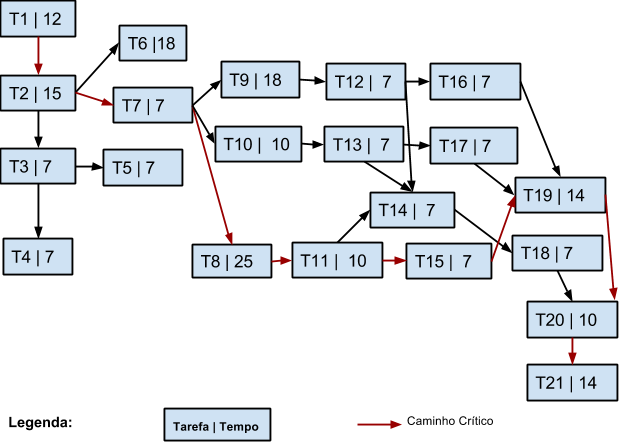
\includegraphics[width=16.722cm,height=11.834cm]{PlanodeProjeto-img002.png} \par}

\bigskip

A partir do caminho crítico mostrado, o tempo mínimo estimado para o projeto é 132 dias úteis.


\bigskip


\bigskip

\clearpage
\subsection{\textcolor[rgb]{0.078431375,0.09411765,0.13725491}{Estimativa de Custo}}\footnote{
\textcolor[rgb]{0.078431375,0.09411765,0.13725491}{O custo foi baseado nos valores disponíveis no seguinte endereço:
}\url{http://info.abril.com.br/noticias/carreira/2014/02/veja-o-salario-de-180-cargos-em-ti.shtml}\par }


\bigskip

\textbf{\textcolor[rgb]{0.078431375,0.09411765,0.13725491}{Custo com profissionais}}


\bigskip

\textcolor[rgb]{0.078431375,0.09411765,0.13725491}{O custo estimado com profissionais é mostrado e detalhado na tabela a
seguir.}


\bigskip


\bigskip

\begin{flushleft}
\tablefirsthead{}
\tablehead{}
\tabletail{}
\tablelasttail{}
\begin{supertabular}{|m{4.428cm}|m{3.476cm}|m{2.074cm}|m{2.4989998cm}|m{2.954cm}|}
\hline
\textbf{\textcolor[rgb]{0.078431375,0.09411765,0.13725491}{Profissional}} &
\textbf{\textcolor[rgb]{0.078431375,0.09411765,0.13725491}{Valor por hora Bruto (R\$)}} &
\textbf{\textcolor[rgb]{0.078431375,0.09411765,0.13725491}{Horas Mensais}} &
\textbf{\textcolor[rgb]{0.078431375,0.09411765,0.13725491}{Salário Mensal Bruto (R\$)}} &
\textbf{\textcolor[rgb]{0.078431375,0.09411765,0.13725491}{Salário Mensal Líquido (R\$)}}\\\hline
\textcolor[rgb]{0.078431375,0.09411765,0.13725491}{Administrador de Banco de Dados Pleno} &
\centering \textcolor[rgb]{0.078431375,0.09411765,0.13725491}{51,4046} &
\centering \textcolor[rgb]{0.078431375,0.09411765,0.13725491}{176} &
\centering \textcolor[rgb]{0.2,0.2,0.2}{9.047,21} &
\centering\arraybslash \textcolor[rgb]{0.2,0.2,0.2}{4.761,69}&\hline
\textcolor[rgb]{0.078431375,0.09411765,0.13725491}{Analista de Sistema Sênior} &
\centering \textcolor[rgb]{0.078431375,0.09411765,0.13725491}{62,0138} &
\centering \textcolor[rgb]{0.078431375,0.09411765,0.13725491}{176} &
\centering 10.914,43 &
\centering\arraybslash 5.744,44&\hline
\textcolor[rgb]{0.078431375,0.09411765,0.13725491}{Analista Programador Júnior} &
\centering \textcolor[rgb]{0.078431375,0.09411765,0.13725491}{26,1124} &
\centering \textcolor[rgb]{0.078431375,0.09411765,0.13725491}{176} &
\centering \textcolor[rgb]{0.2,0.2,0.2}{4.595,79} &
\centering\arraybslash \textcolor[rgb]{0.2,0.2,0.2}{2.418,84}&\hline
\textcolor[rgb]{0.078431375,0.09411765,0.13725491}{Analista Programador Pleno} &
\centering \textcolor[rgb]{0.078431375,0.09411765,0.13725491}{41,3600} &
\centering \textcolor[rgb]{0.078431375,0.09411765,0.13725491}{176} &
\centering \textcolor[rgb]{0.2,0.2,0.2}{7.279,37} &
\centering\arraybslash \textcolor[rgb]{0.2,0.2,0.2}{3.831,25}&\hline
\textcolor[rgb]{0.078431375,0.09411765,0.13725491}{Analista Programador Sênior} &
\centering \textcolor[rgb]{0.078431375,0.09411765,0.13725491}{58,1506} &
\centering \textcolor[rgb]{0.078431375,0.09411765,0.13725491}{176} &
\centering \textcolor[rgb]{0.2,0.2,0.2}{10.234,52} &
\centering\arraybslash \textcolor[rgb]{0.2,0.2,0.2}{5.386,59}&\hline
\textcolor[rgb]{0.078431375,0.09411765,0.13725491}{Designer Pleno} &
\centering \textcolor[rgb]{0.078431375,0.09411765,0.13725491}{21,6219} &
\centering \textcolor[rgb]{0.078431375,0.09411765,0.13725491}{176} &
\centering \textcolor[rgb]{0.2,0.2,0.2}{3.805,47} &
\centering\arraybslash \textcolor[rgb]{0.2,0.2,0.2}{2.002,88}&\hline
\textcolor[rgb]{0.078431375,0.09411765,0.13725491}{Testador Pleno} &
\centering \textcolor[rgb]{0.078431375,0.09411765,0.13725491}{32,7917} &
\centering \textcolor[rgb]{0.078431375,0.09411765,0.13725491}{176} &
\centering \textcolor[rgb]{0.2,0.2,0.2}{5.771,34} &
\centering\arraybslash \textcolor[rgb]{0.2,0.2,0.2}{3.037,55}&\hline
\end{supertabular}
\end{flushleft}
\liststyleWWNumii
\begin{itemize}
\item \textcolor[rgb]{0.078431375,0.09411765,0.13725491}{Assumindo que o valor dos impostos acumula 90\% sobre o salário
bruto de cada funcionário.}
\end{itemize}

\bigskip

\textbf{\textcolor[rgb]{0.078431375,0.09411765,0.13725491}{Custo com equipamento}}\footnote{ Valores dos
computadores retirados do site da Dell, Kabum, Saraiva}

\textcolor[rgb]{0.078431375,0.09411765,0.13725491}{O custo com equipamentos foi estimado de acordo com a quantidade de
produtos que serão comprados e os respectivos preços na data de escrita deste documento. Esse custo compreende os
seguintes equipamentos: 5 computadores de mesa, 5 computadores portáteis), 1 livro de banco de dados para consulta, 1
livro de programação mobile para consulta, 1}\textit{\textcolor[rgb]{0.078431375,0.09411765,0.13725491}{
tablet}}\textcolor[rgb]{0.078431375,0.09411765,0.13725491}{ para teste do módulo do garçom. Os valores desses
equipamentos são detalhados na tabela a seguir.}


\bigskip

\begin{flushleft}
\tablefirsthead{}
\tablehead{}
\tabletail{}
\tablelasttail{}
\begin{supertabular}{|m{4.984cm}|m{3.9799998cm}|m{2.7619998cm}|m{4.564cm}|}
\hline
\centering \textbf{\textcolor[rgb]{0.078431375,0.09411765,0.13725491}{Produto}} &
\centering \textbf{\textcolor[rgb]{0.078431375,0.09411765,0.13725491}{Valor unitário(R\$)}} &
\centering \textbf{\textcolor[rgb]{0.078431375,0.09411765,0.13725491}{Quantidade}} &
\centering\arraybslash \textbf{\textcolor[rgb]{0.078431375,0.09411765,0.13725491}{Custo (R\$)}}&\hline
\centering \textcolor[rgb]{0.078431375,0.09411765,0.13725491}{Computador de mesa} &
\centering \textcolor[rgb]{0.078431375,0.09411765,0.13725491}{1.500} &
\centering \textcolor[rgb]{0.078431375,0.09411765,0.13725491}{5} &
\centering\arraybslash \textcolor[rgb]{0.078431375,0.09411765,0.13725491}{7.500}&\hline
\centering \textcolor[rgb]{0.078431375,0.09411765,0.13725491}{Computador portátil} &
\centering \textcolor[rgb]{0.078431375,0.09411765,0.13725491}{1.600} &
\centering \textcolor[rgb]{0.078431375,0.09411765,0.13725491}{5} &
\centering\arraybslash \textcolor[rgb]{0.078431375,0.09411765,0.13725491}{8.000}&\hline
\centering \textcolor[rgb]{0.078431375,0.09411765,0.13725491}{Tablets} &
\centering \textcolor[rgb]{0.078431375,0.09411765,0.13725491}{800} &
\centering \textcolor[rgb]{0.078431375,0.09411765,0.13725491}{1} &
\centering\arraybslash \textcolor[rgb]{0.078431375,0.09411765,0.13725491}{800}&\hline
\centering \textcolor[rgb]{0.078431375,0.09411765,0.13725491}{Livros} &
\centering \textcolor[rgb]{0.078431375,0.09411765,0.13725491}{150} &
\centering \textcolor[rgb]{0.078431375,0.09411765,0.13725491}{2} &
\centering\arraybslash \textcolor[rgb]{0.078431375,0.09411765,0.13725491}{300}&\hline
\centering \textbf{\textcolor[rgb]{0.078431375,0.09411765,0.13725491}{Total}} &
\centering \textbf{\textcolor[rgb]{0.078431375,0.09411765,0.13725491}{4.050,00}} &
\centering \textbf{\textcolor[rgb]{0.078431375,0.09411765,0.13725491}{13}} &
\centering\arraybslash \textbf{\textcolor[rgb]{0.078431375,0.09411765,0.13725491}{16.600,00}}&\hline
\end{supertabular}
\end{flushleft}

\bigskip


\bigskip

\textbf{\textcolor[rgb]{0.078431375,0.09411765,0.13725491}{Custo com treinamento}}

\textcolor[rgb]{0.078431375,0.09411765,0.13725491}{Para adaptação dos programadores as tecnologias usadas no projeto, o
programador sênior fará um treinamento dos analistas programadores júnior durante a fase de levantamento de requisitos
e modelagem do projeto. Esse treinamento deve ser feito obrigatoriamente até o fim da tarefa 2 e somente haverá
treinamento dos profissionais de nível pleno, caso este profissional seja contratado sem passar pelo mesmo cargo de
nível júnior na empresa. Ou seja, não haverá custo extra com o treinamento já que esse profissional que fará o
treinamento estará recebendo o seu salário para essa função.}


\bigskip


\bigskip

\textbf{\textcolor[rgb]{0.078431375,0.09411765,0.13725491}{Custo com ambiente}}

\textcolor[rgb]{0.078431375,0.09411765,0.13725491}{Para o desenvolvimento do sistema, é necessária a aquisição ou
aluguel de um imóvel onde a equipe trabalhará. Foi estabelecido um valor de R\$ 900 mensais para o aluguel de uma sala
durante o tempo estimado no item 4, que foi de 132 dias. Com isso, o valor total estimado foi de R\$5.400,00.}


\bigskip

\textbf{\textcolor[rgb]{0.078431375,0.09411765,0.13725491}{Custo Total}}


\bigskip

\begin{flushleft}
\tablefirsthead{}
\tablehead{}
\tabletail{}
\tablelasttail{}
\begin{supertabular}{|m{13.213cm}|m{2.816cm}|}
\hline
\textbf{\textcolor[rgb]{0.078431375,0.09411765,0.13725491}{Tipo de custo}} &
\centering\arraybslash \textbf{\textcolor[rgb]{0.078431375,0.09411765,0.13725491}{\ Custo (R\$)}}&\hline
\textcolor[rgb]{0.078431375,0.09411765,0.13725491}{Custo com funcionários} &
\raggedleft\arraybslash \textcolor[rgb]{0.078431375,0.09411765,0.13725491}{222.307,7432}&\hline
\textcolor[rgb]{0.078431375,0.09411765,0.13725491}{Equipamentos} &
\raggedleft\arraybslash \textcolor[rgb]{0.078431375,0.09411765,0.13725491}{16.600,00}&\hline
\textcolor[rgb]{0.078431375,0.09411765,0.13725491}{Ambiente} &
\raggedleft\arraybslash \textcolor[rgb]{0.078431375,0.09411765,0.13725491}{5.400,00}&\hline
\textbf{\textcolor[rgb]{0.078431375,0.09411765,0.13725491}{Total}} &
\raggedleft\arraybslash \textbf{\textcolor[rgb]{0.078431375,0.09411765,0.13725491}{244.307,74}}&\hline
\end{supertabular}
\end{flushleft}

\bigskip

\clearpage
\section{Casos de Uso}
\textbf{Nome:} Cadastrar funcionário.

\textbf{Descrição:} Cadastra um funcionário no sistema.

\textbf{Identificador: CDU1}

\textbf{Importância: 4}

\textbf{Ator Primário: }Gerente.

\textbf{Fluxo Principal:}

\begin{flushleft}
\tablefirsthead{}
\tablehead{}
\tabletail{}
\tablelasttail{}
\begin{supertabular}{|m{8.212cm}|m{7.9490004cm}|}
\hline
Gerente &
Sistema\\\hline
1 - Insere os dados \ do funcionário no sistema  &
~
\\\hline
~
 &
2 - Registra os dados\\\hline
~
 &
3 - Confirma operação\\\hline
\end{supertabular}
\end{flushleft}

\bigskip

\textbf{Nome:} Alterar funcionário

\textbf{Descrição:} Altera as informações de um funcionário no sistema.

\textbf{Identificador: CDU2}

\textbf{Importância: 3}

\textbf{Ator Primário: }Gerente.

\textbf{Pré-condições: }O funcionário deve está cadastrado no sistema.

\textbf{Fluxo Principal:}

\begin{flushleft}
\tablefirsthead{}
\tablehead{}
\tabletail{}
\tablelasttail{}
\begin{supertabular}{|m{8.265cm}|m{7.7380004cm}|}
\hline
Gerente &
Sistema\\\hline
1 - Solicita o registro do funcionário ao sistema &
~
\\\hline
~
 &
2a - Retorna o registro do funcionário.

2b - Retorna aviso que o funcionário não se encontra no sistema\\\hline
3 - Altera os dados do funcionário no sistema  &
~
\\\hline
~
 &
4 - Registra os dados do funcionário \\\hline
~
 &
5 - Confirma operação \\\hline
\end{supertabular}
\end{flushleft}

\bigskip


\bigskip


\bigskip

\textbf{Nome:} Demitir funcionário

\textbf{Descrição:} Remove cadastro do funcionário associado ao sistema.

\textbf{Identificador: CDU3}

\textbf{Importância: 3}

\textbf{Ator Primário: }Gerente.

\textbf{Pré-condições: }O\textbf{ }funcionário deve estar cadastrado no sistema e deve não estar associado a qualquer
escala de horário do sistema.

\textbf{Fluxo Principal: }

\begin{flushleft}
\tablefirsthead{}
\tablehead{}
\tabletail{}
\tablelasttail{}
\begin{supertabular}{|m{7.974cm}|m{7.8170004cm}|}
\hline
Gerente &
Sistema\\\hline
1 - Solicita o registro do funcionário ao sistema &
~
\\\hline
~
 &
2a - Retorna o registro do funcionário

2b - Retorna aviso que o funcionário não se encontra no sistema\\\hline
3 - Solicita remoção do funcionário ao sistema &
~
\\\hline
~
 &
4 - Exclui funcionário do sistema\\\hline
~
 &
5 - Confirma operação\\\hline
\end{supertabular}
\end{flushleft}

\bigskip

\textbf{Nome:} Registrar hora extra.

\textbf{Descrição:} Registra as horas extras dos funcionários.

\textbf{Identificador: CDU4}

\textbf{Importância: 2}

\textbf{Ator Primário: }Gerente.

\textbf{Pré-condições: }O funcionário deve está cadastrado no sistema.

\textbf{Fluxo Principal:}

\begin{flushleft}
\tablefirsthead{}
\tablehead{}
\tabletail{}
\tablelasttail{}
\begin{supertabular}{|m{7.471cm}|m{7.05cm}|}
\hline
Gerente &
Sistema\\\hline
1 - Solicita o registro do funcionário ao sistema &
~
\\\hline
~
 &
2a - Retorna o registro do funcionário

2b - Retorna aviso que o funcionário não se encontra no sistema\\\hline
3 - Insere as horas extras no sistema &
~
\\\hline
~
 &
4 - Registra as horas extras do funcionário \\\hline
~
 &
5 - Confirma operação\\\hline
\end{supertabular}
\end{flushleft}

\bigskip


\bigskip

\textbf{Nome:} Cadastrar Escala de Horários.

\textbf{Descrição:} Cadastra as escalas de horários dos funcionários.

\textbf{Identificador: CDU5}

\textbf{Importância: 4}

\textbf{Ator Primário: }Gerente.

\textbf{Pré-condições: }O funcionário deve está cadastrado no sistema.

\textbf{Fluxo Principal:}

\begin{flushleft}
\tablefirsthead{}
\tablehead{}
\tabletail{}
\tablelasttail{}
\begin{supertabular}{|m{7.8150005cm}|m{7.9490004cm}|}
\hline
Gerente &
Sistema\\\hline
1 - Informa turno de trabalho &
~
\\\hline
2 - Solicita escala de horários ao sistema &
~
\\\hline
~
 &
3 - Retorna escala de horários\\\hline
4 - Aloca funcionário na escala de horário &
~
\\\hline
~
 &
5 - Registra alocação de horário \\\hline
~
 &
6 - Confirma operação\\\hline
\end{supertabular}
\end{flushleft}

\bigskip

\textbf{Nome:} Alterar Escala de Horários

\textbf{Descrição:} Altera as escalas de horários dos funcionários.

\textbf{Identificador: CDU6}

\textbf{Importância: 1}

\textbf{Ator Primário: }Gerente.

\textbf{Pré-condições: }O funcionário deve está cadastrado no sistema.

\textbf{Fluxo Principal:}

\begin{flushleft}
\tablefirsthead{}
\tablehead{}
\tabletail{}
\tablelasttail{}
\begin{supertabular}{|m{7.683cm}|m{8.055cm}|}
\hline
Gerente &
Sistema\\\hline
1 -Solicita escala de horários ao sistema &
~
\\\hline
~
 &
2 - Retorna escala de horários\\\hline
3 - Altera a escala de horários do funcionário &
~
\\\hline
~
 &
4 - Registra a nova escala de horário\\\hline
~
 &
5 - Confirma operação\\\hline
\end{supertabular}
\end{flushleft}

\bigskip

\textbf{Nome:} Cadastrar desconto.

\textbf{Descrição:} Cadastra descontos.

\textbf{Identificador: CDU7}

\textbf{Importância: 3}

\textbf{Ator Primário: }Gerente.

\textbf{Pré-condições: }Devem existir refeições cadastradas.

\textbf{Fluxo Principal:}

\begin{flushleft}
\tablefirsthead{}
\tablehead{}
\tabletail{}
\tablelasttail{}
\begin{supertabular}{|m{7.87cm}|m{7.868cm}|}
\hline
Gerente &
Sistema\\\hline
1 - Consulta refeições &
~
\\\hline
~
 &
2 - Retorna as refeições\\\hline
3 - Associa refeições a um desconto &
~
\\\hline
~
 &
4 - Registra desconto\\\hline
~
 &
5 - Confirma operação\\\hline
\end{supertabular}
\end{flushleft}

\bigskip

\textbf{Nome:} Alterar desconto.

\textbf{Descrição:} O gerente altera o desconto.

\textbf{Identificador: CDU8}

\textbf{Importância: 3}

\textbf{Ator Primário: }Gerente.

\textbf{Pré-condições: }O desconto deve existir.

\textbf{Fluxo Principal:}

\begin{flushleft}
\tablefirsthead{}
\tablehead{}
\tabletail{}
\tablelasttail{}
\begin{supertabular}{|m{7.974cm}|m{7.7380004cm}|}
\hline
Gerente &
Sistema\\\hline
1 - Solicita registro desconto &
~
\\\hline
~
 &
2 - Retorna registro do desconto\\\hline
3 - Altera informações do desconto &
~
\\\hline
~
 &
5 - Registra desconto\\\hline
~
 &
6 - Confirma operação\\\hline
\end{supertabular}
\end{flushleft}

\bigskip

\textbf{Nome:} Excluir desconto.

\textbf{Descrição: }O gerente remove o desconto.

\textbf{Identificador: CDU9}

\textbf{Importância: 3}

\textbf{Ator Primário: }Gerente.

\textbf{Pré-condições: }O desconto deve existir.

\textbf{Fluxo Principal:}

\begin{flushleft}
\tablefirsthead{}
\tablehead{}
\tabletail{}
\tablelasttail{}
\begin{supertabular}{|m{7.894cm}|m{7.7640004cm}|}
\hline
Gerente &
Sistema\\\hline
1 - Solicita registro do desconto &
~
\\\hline
~
 &
2 - Retorna registro do desconto\\\hline
3 - Exclui desconto &
~
\\\hline
4 - Confirma exclusão. &
~
\\\hline
~
 &
5 - Realiza exclusão\\\hline
~
 &
6 - Confirma operação\\\hline
\end{supertabular}
\end{flushleft}

\bigskip

\textbf{Nome:} Cadastrar Item.

\textbf{Descrição:} O estoquista cadastra um novo item no sistema.

\textbf{Identificador: CDU10}

\textbf{Importância: 4}

\textbf{Ator Principal:} Estoquista.

\textbf{Fluxo Principal:}

\begin{flushleft}
\tablefirsthead{}
\tablehead{}
\tabletail{}
\tablelasttail{}
\begin{supertabular}{|m{7.709cm}|m{8.108cm}|}
\hline
Estoquista &
Sistema\\\hline
1 - Informa ao sistema o item a ser cadastrado &
~
\\\hline
~
 &
2 - Registra cadastro\\\hline
~
 &
3 - Confirma operação\\\hline
\end{supertabular}
\end{flushleft}

\bigskip

\textbf{Nome:} Alterar Item.

\textbf{Descrição:} Altera um determinado item no sistema.

\textbf{Identificador: CDU11}

\textbf{Importância: 3}

\textbf{Ator Principal:} Estoquista.

\textbf{Pré-condições: }O Item deve existir.

\textbf{Fluxo Principal:}

\begin{flushleft}
\tablefirsthead{}
\tablehead{}
\tabletail{}
\tablelasttail{}
\begin{supertabular}{|m{7.656cm}|m{7.87cm}|}
\hline
Estoquista &
Sistema\\\hline
1 - Consulta o item no sistema &
~
\\\hline
~
 &
2 - Retorna o registro do item.\\\hline
3 - Realiza alterações &
~
\\\hline
4 - Confirma alterações &
~
\\\hline
~
 &
5 - Registra alterações\\\hline
~
 &
6 - Confirma operação\\\hline
\end{supertabular}
\end{flushleft}

\bigskip

\textbf{Nome:} Excluir Item.

\textbf{Descrição:} O estoquista exclui o item no sistema.

\textbf{Identificador: CDU12}

\textbf{Importância: 3}

\textbf{Ator Principal:} Estoquista.

\textbf{Pré-condições: }O Item deve existir.

\textbf{Fluxo Principal:}


\bigskip

\begin{flushleft}
\tablefirsthead{}
\tablehead{}
\tabletail{}
\tablelasttail{}
\begin{supertabular}{|m{7.471cm}|m{8.055cm}|}
\hline
Estoquista &
Sistema\\\hline
1 - Consulta item no sistema. &
~
\\\hline
~
 &
2 - Retorna o registro do item.\\\hline
3 - Exclui item &
~
\\\hline
4 - Confirma exclusão. &
~
\\\hline
~
 &
5 - Realiza exclusão\\\hline
~
 &
6 - Confirma operação\\\hline
\end{supertabular}
\end{flushleft}

\bigskip

\textbf{Nome:} Consultar Item.

\textbf{Descrição:} O estoquista consulta item no sistema.

\textbf{Identificador: CDU13}

\textbf{Importância: 3}

\textbf{Ator Principal:} Estoquista.

\textbf{Fluxo Principal:}


\bigskip

\begin{flushleft}
\tablefirsthead{}
\tablehead{}
\tabletail{}
\tablelasttail{}
\begin{supertabular}{|m{7.392cm}|m{8.134cm}|}
\hline
Estoquista &
Sistema\\\hline
1 - Informa ao sistema item escolhido &
~
\\\hline
~
 &
2a - Retorna o registro do item.

2b - Retorna aviso que o item não se encontra no sistema\\\hline
3 - Visualiza item consultado &
~
\\\hline
\end{supertabular}
\end{flushleft}

\bigskip

\textbf{Nome:} Cadastrar fornecedor.

\textbf{Descrição:} Cria o cadastro de um fornecedor no sistema.

\textbf{Identificador: CDU14}

\textbf{Importância: 5}

\textbf{Ator Primário: }Estoquista.

\textbf{Fluxo Principal:}

\begin{flushleft}
\tablefirsthead{}
\tablehead{}
\tabletail{}
\tablelasttail{}
\begin{supertabular}{|m{7.3650002cm}|m{8.214cm}|}
\hline
Estoquista &
Sistema\\\hline
1 - Informa ao sistema dados do fornecedor a ser cadastrado &
~
\\\hline
~
 &
2 - Registra fornecedor\\\hline
~
 &
3 - Confirma operação\\\hline
\end{supertabular}
\end{flushleft}

\bigskip


\bigskip

\textbf{Nome:} Alterar fornecedor.

\textbf{Descrição:} Altera informações do cadastro de um fornecedor no sistema.

\textbf{Identificador: CDU15}

\textbf{Importância: 3}

\textbf{Ator Primário: }Estoquista.

\textbf{Pré- Condições:} O fornecedor deve estar cadastrado no sistema.

\textbf{Fluxo Principal:}

\begin{flushleft}
\tablefirsthead{}
\tablehead{}
\tabletail{}
\tablelasttail{}
\begin{supertabular}{|m{7.524cm}|m{8.055cm}|}
\hline
Estoquista &
Sistema\\\hline
1 - Solicita o registro do fornecedor ao sistema &
~
\\\hline
~
 &
2 - Retorna o registro do fornecedor.\\\hline
3 - Altera os dados do fornecedor no sistema  &
~
\\\hline
~
 &
4 - Registra os dados do fornecedor \\\hline
~
 &
5 - Confirma cadastro do fornecedor \\\hline
\end{supertabular}
\end{flushleft}

\bigskip

\textbf{Nome:} Excluir fornecedor.

\textbf{Descrição:} Exclui um fornecedor do sistema.

\textbf{Identificador: CDU16}

\textbf{Importância: 4}

\textbf{Ator Primário: }Estoquista.

\textbf{Pré- Condições:} Fornecedor deve estar cadastrado no sistema.

\textbf{Fluxo Principal:}

\begin{flushleft}
\tablefirsthead{}
\tablehead{}
\tabletail{}
\tablelasttail{}
\begin{supertabular}{|m{7.551cm}|m{7.9490004cm}|}
\hline
Estoquista &
Sistema\\\hline
1 - Consulta o fornecedor no sistema &
~
\\\hline
~
 &
2 - Retorna o registro do fornecedor.\\\hline
3 - Exclui o fornecedor &
~
\\\hline
4 - Confirma exclusão &
~
\\\hline
~
 &
5 - Realiza exclusão\\\hline
~
 &
6 - Confirma operação\\\hline
\end{supertabular}
\end{flushleft}

\bigskip

\textbf{Nome:} Consultar fornecedor.

\textbf{Descrição:} Faz uma consulta nos fornecedores cadastrados no sistema.

\textbf{Identificador: CDU17}

\textbf{Importância: 3}

\textbf{Ator Primário: }Estoquista.

\textbf{Fluxo Principal:}

\begin{flushleft}
\tablefirsthead{}
\tablehead{}
\tabletail{}
\tablelasttail{}
\begin{supertabular}{|m{7.471cm}|m{8.029cm}|}
\hline
Estoquista &
Sistema\\\hline
1 - Informa ao sistema o fornecedor a ser consultado. &
~
\\\hline
~
 &
2a - Retorna o registro do fornecedor.

2b - Retorna aviso que o fornecedor não se encontra no sistema\\\hline
3 - Visualiza a consulta. &
~
\\\hline
\end{supertabular}
\end{flushleft}

\bigskip


\bigskip

\textbf{Nome:} Consultar refeição.

\textbf{Descrição:} O Garçom consulta no sistema as refeições disponíveis.

\textbf{Identificador: CDU18}

\textbf{Importância: 4}

\textbf{Ator Principal:} Garçom.

\textbf{Fluxo Principal:}

\begin{flushleft}
\tablefirsthead{}
\tablehead{}
\tabletail{}
\tablelasttail{}
\begin{supertabular}{|m{7.524cm}|m{8.029cm}|}
\hline
Garçom &
Sistema\\\hline
1 - Informa ao sistema a refeição a ser consultada &
~
\\\hline
~
 &
2a - Retorna o registro da refeição.

2b - Retorna um aviso que a refeição não está cadastrada no sistema.\\\hline
3- Visualiza a refeição &
~
\\\hline
\end{supertabular}
\end{flushleft}

\bigskip

\textbf{Nome:} Cadastrar refeição.

\textbf{Descrição:} Cadastra uma refeição no sistema.

\textbf{Identificador: CDU19}

\textbf{Importância: 5}

\textbf{Ator Primário: }Gerente.

\textbf{Fluxo Principal:}

\begin{flushleft}
\tablefirsthead{}
\tablehead{}
\tabletail{}
\tablelasttail{}
\begin{supertabular}{|m{7.709cm}|m{7.8430004cm}|}
\hline
Gerente &
Sistema\\\hline
1 - Informa ao sistema a refeição a ser cadastrada. &
~
\\\hline
~
 &
2 - Registra refeição\\\hline
~
 &
3 - Confirma operação\\\hline
\end{supertabular}
\end{flushleft}

\bigskip


\bigskip

\textbf{Nome:} Alterar refeição.

\textbf{Descrição:} Altera o cadastro de uma refeição no sistema.

\textbf{Identificador: CDU20}

\textbf{Impo\ \ rtância: 4}

\textbf{Ator Primário: }Gerente.

\textbf{Pré- Condições:} A refeição deve estar cadastrada no sistema.

\textbf{Fluxo Principal:}


\bigskip

\begin{flushleft}
\tablefirsthead{}
\tablehead{}
\tabletail{}
\tablelasttail{}
\begin{supertabular}{|m{7.5490003cm}|m{7.977cm}|}
\hline
Gerente &
Sistema\\\hline
1 - Consulta refeição no sistema &
~
\\\hline
~
 &
2 - Retorna o registro da refeição.\\\hline
3 - Realiza alterações &
~
\\\hline
4 - Confirma alterações &
~
\\\hline
~
 &
5 - Registra alterações\\\hline
~
 &
6 - Confirma operação\\\hline
\end{supertabular}
\end{flushleft}

\bigskip

\textbf{Nome:} Excluir refeição.

\textbf{Descrição:} Exclui o cadastro de uma refeição no sistema.

\textbf{Identificador: CDU21}

\textbf{Importância: 3}

\textbf{Ator Primário: }Gerente.

\textbf{Pré- Condições:} A refeição deve estar cadastrada no sistema.

\textbf{Fluxo Principal:}


\bigskip

\begin{flushleft}
\tablefirsthead{}
\tablehead{}
\tabletail{}
\tablelasttail{}
\begin{supertabular}{|m{7.498cm}|m{8.002cm}|}
\hline
Gerente &
Sistema\\\hline
1 - Consulta refeição no sistema &
~
\\\hline
~
 &
2 - Retorna o registro da refeição.\\\hline
3 - Exclui refeição &
~
\\\hline
4 - Confirma exclusão &
~
\\\hline
~
 &
5 - Realiza exclusão\\\hline
~
 &
6 - Confirma operação\\\hline
\end{supertabular}
\end{flushleft}

\bigskip

\textbf{Nome}: Incluir Pedido na Comanda.

\textbf{Descrição:} O Garçom inclui o pedido do Cliente na comanda referente à mesa deste Cliente.

\textbf{Identificador: CDU22}

\textbf{Importância: 5}

\textbf{Ator Principal:} Garçom

\textbf{Pré- Condições:} Comanda da mesa deve ter sido incluída.

\textbf{Fluxo Principal:}

\begin{flushleft}
\tablefirsthead{}
\tablehead{}
\tabletail{}
\tablelasttail{}
\begin{supertabular}{|m{7.418cm}|m{8.081cm}|}
\hline
Garçom &
Sistema\\\hline
1 - Consulta comanda no sistema. &
~
\\\hline
~
 &
2 - Retorna comanda consultada\\\hline
3 - Insere o pedido no sistema. &
~
\\\hline
~
 &
4 - Registra o pedido\\\hline
5 - Inclui o pedido na comanda. &
~
\\\hline
~
 &
6 - Realiza Inclusão\\\hline
~
 &
7 - Confirma inclusão\\\hline
\end{supertabular}
\end{flushleft}

\bigskip

\textbf{Nome: }Excluir pedido da comanda.

\textbf{Descrição: }O Garçom remove o pedido da comanda mediante solicitação do Cliente.

\textbf{Identificador: CDU23}

\textbf{Importância: 3}

\textbf{Ator Principal: }Garçom.

\textbf{Pré- Condições:} O pedido deve ter sido incluído na comanda.

\textbf{Fluxo Principal:}

\begin{flushleft}
\tablefirsthead{}
\tablehead{}
\tabletail{}
\tablelasttail{}
\begin{supertabular}{|m{7.3120003cm}|m{8.108cm}|}
\hline
Garçom &
Sistema\\\hline
\ 1- Consulta a comanda no sistema. &
~
\\\hline
~
 &
2 - Retorna a comanda consultada\\\hline
3- Solicita pedido a ser removido da comanda. &
~
\\\hline
~
 &
4 - Retorna pedido\\\hline
5 - Exclui pedido da comanda &
~
\\\hline
~
 &
6 - Realiza Exclusão\\\hline
~
 &
7 - Confirma Exclusão\\\hline
\end{supertabular}
\end{flushleft}

\bigskip

\textbf{Nome: }Incluir comanda

\textbf{Descrição: }O Garçom cria uma comanda ativa associada a um cliente.

\textbf{Identificador: CDU24}

\textbf{Importância: 5}

\textbf{Ator Principal: }Garçom.

\textbf{Fluxo Principal:}

\begin{flushleft}
\tablefirsthead{}
\tablehead{}
\tabletail{}
\tablelasttail{}
\begin{supertabular}{|m{7.551cm}|m{7.9230003cm}|}
\hline
Garçom &
Sistema\\\hline
1- Solicita ao sistema o inicio de uma nova comanda. &
~
\\\hline
~
 &
2 - Inclui uma nova comanda.\\\hline
\end{supertabular}
\end{flushleft}

\bigskip

\textbf{Nome:} Pagar comanda.

\textbf{Descrição:} É efetuado o pagamento da comanda.

\textbf{Identificador: CDU25}

\textbf{Importância: 5}

\textbf{Ator Principal:} Garçom.

\textbf{Pré- Condições:} A comanda deve ter sido incluída e estar ativa.

\textbf{Fluxo Principal:} 

\begin{flushleft}
\tablefirsthead{}
\tablehead{}
\tabletail{}
\tablelasttail{}
\begin{supertabular}{|m{7.603cm}|m{7.896cm}|}
\hline
Garçom &
Sistema\\\hline
1- Consulta a comanda no sistema. &
~
\\\hline
~
 &
2 - Retorna comanda\\\hline
3 - Solicita finalização da comanda. &
~
\\\hline
~
 &
4 - Finaliza comanda\\\hline
~
 &
5 - Imprime a conta\\\hline
6 - Informa ao sistema a forma de pagamento escolhida pelo cliente &
~
\\\hline
~
 &
7 - Registra pagamento\\\hline
~
 &
8 - Imprime cupom fiscal\\\hline
\end{supertabular}
\end{flushleft}

\bigskip

\textbf{Nome:} Consultar comanda.

\textbf{Descrição:} O Garçom consulta no sistema por uma comanda de uma mesa específica.

\textbf{Identificador: CDU26}

\textbf{Importância: 1}

\textbf{Ator Principal:} Garçom.

\textbf{Fluxo Principal:}

\begin{flushleft}
\tablefirsthead{}
\tablehead{}
\tabletail{}
\tablelasttail{}
\begin{supertabular}{|m{7.656cm}|m{7.8170004cm}|}
\hline
Garçom &
Sistema\\\hline
1- Informa ao sistema qual mesa deseja consultar &
~
\\\hline
~
 &
2 - Retorna as informações da mesa desejada\\\hline
3 - Recebe a informação solicitada ao sistema &
~
\\\hline
\end{supertabular}
\end{flushleft}

\bigskip

\textbf{Nome:} Gerar Comandas.

\textbf{Descrição:} O garçom solicita a geração de comandas.

\textbf{Identificador: CDU27}

\textbf{Importância: 5}

\textbf{Ator Principal:} Garçom.

\textbf{Fluxo Principal:}

\begin{flushleft}
\tablefirsthead{}
\tablehead{}
\tabletail{}
\tablelasttail{}
\begin{supertabular}{|m{7.551cm}|m{7.9490004cm}|}
\hline
Garçom &
Sistema\\\hline
1- Solicita a geração de comanda no sistema &
~
\\\hline
~
 &
2- \ Gera a comanda\\\hline
\end{supertabular}
\end{flushleft}

\bigskip

\textbf{Nome:} Gerar Relatório

\textbf{Descrição:} O funcionário gera os relatórios .

\textbf{Identificador: CDU28}

\textbf{Importância: 4}

\textbf{Ator Principal:} Funcionário.

\textbf{Fluxo Principal:}

\begin{flushleft}
\tablefirsthead{}
\tablehead{}
\tabletail{}
\tablelasttail{}
\begin{supertabular}{|m{7.471cm}|m{8.029cm}|}
\hline
Funcionário &
Sistema\\\hline
1 - Solicita os tipos de relatórios &
~
\\\hline
~
 &
2 - Informa opções de relatórios\\\hline
3 - Seleciona o relatório desejado &
~
\\\hline
~
 &
4 - Gera o relatório\\\hline
\end{supertabular}
\end{flushleft}

\bigskip


\bigskip


\bigskip


\bigskip
\section{Código Projeto}
\subsection{Model}
\subsubsection{Comanda}
\lstinputlisting{model/comanda.rb}
\subsubsection{Componentes produtos}
\lstinputlisting{model/componentes_produto.rb}
\subsubsection{Fornecedor}
\lstinputlisting{model/fornecedor.rb}
\subsubsection{Funcionario}
\lstinputlisting{model/funcionario.rb}
\subsubsection{Item}
\lstinputlisting{model/item.rb}
\subsubsection{Pedido}
\lstinputlisting{model/pedido.rb}
\subsubsection{Produto}
\lstinputlisting{model/produto.rb}
\subsubsection{Vende}
\lstinputlisting{model/vende.rb}
  \newpage
  
\subsection{View}
\setcounter{secnumdepth}{4}
\subsubsection{Comanda}
\paragraph{Form}
\lstinputlisting{view/comanda/form.html.erb}
\paragraph{Editar}
\lstinputlisting{view/comanda/edit.html.erb}
\paragraph{Index}
\lstinputlisting{view/comanda/index.html.erb}
\paragraph{Index json}
\lstinputlisting{view/comanda/index.json.jbuilder}
\paragraph{Novo}
\lstinputlisting{view/comanda/new.html.erb}
\paragraph{Visualizar}
\lstinputlisting{view/comanda/show.html.erb}
\paragraph{Visualizar json}
\lstinputlisting{view/comanda/show.json.jbuilder}


\subsubsection{Compra}
\paragraph{Form}
\lstinputlisting{view/compra/_form.html.erb}
\paragraph{Item}
\lstinputlisting{view/compra/_item_form.html.erb}
\paragraph{Tabela Itens}
\lstinputlisting{view/compra/_item_table.html.erb}
\paragraph{Editar}
\lstinputlisting{view/compra/edit.html.erb}
\paragraph{Index}
\lstinputlisting{view/compra/index.html.erb}
\paragraph{Index json}
\lstinputlisting{view/compra/index.json.jbuilder}
\paragraph{Editar Item}
\lstinputlisting{view/compra/item_edit.html.erb}
\paragraph{Item index}
\lstinputlisting{view/compra/item_index.html.erb}
\paragraph{Item index json}
\lstinputlisting{view/compra/item_index.json.jbuilder}
\paragraph{Novo Item}
\lstinputlisting{view/compra/item_new.html.erb}
\paragraph{Consultar Item}
\lstinputlisting{view/compra/item_search.html.erb}
\paragraph{Visualizar Item}
\lstinputlisting{view/compra/item_show.html.erb}
\paragraph{Item show json}
\lstinputlisting{view/compra/item_show.json.jbuilder}
\paragraph{Novo}
\lstinputlisting{view/compra/new.html.erb}
\paragraph{Relatorio itens em falta}
\lstinputlisting{view/compra/relatorio_itens_falta.html.erb}
\paragraph{Visualizar}
\lstinputlisting{view/compra/show.html.erb}
\paragraph{Visualizar json}
\lstinputlisting{view/compra/show.json.jbuilder}


\subsubection{Fornecedor}
\paragraph{Form}
\lstinputlisting{view/fornecedor/_form.html.erb}
\paragraph{Lista de itens}
\lstinputlisting{view/fornecedor/_list_items.html.erb}
\paragraph{Tabela}
\lstinputlisting{view/fornecedor/_table.html.erb}
\paragraph{Editar}
\lstinputlisting{view/fornecedor/edit.html.erb}
\paragraph{Index}
\lstinputlisting{view/fornecedor/index.html.erb}
\paragraph{Index json}
\lstinputlisting{view/fornecedor/index.json.jbuilder}
\paragraph{Novo}
\lstinputlisting{view/fornecedor/new.html.erb}
\paragraph{Relatório}
\lstinputlisting{view/fornecedor/relatorio.html.erb}
\paragraph{Buscar}
\lstinputlisting{view/fornecedor/search.html.erb}
\paragraph{Visualizar}
\lstinputlisting{view/fornecedor/show.html.erb}
\paragraph{Visualizar json}
\lstinputlisting{view/fornecedor/show.json.jbuilder}

\subsubsection{Funcionario}
\paragraph{Form}
\lstinputlisting{view/funcionario/_form.html.erb}
\paragraph{Tabela}
\lstinputlisting{view/funcionario/_table.html.erb}
\paragraph{Editar}
\lstinputlisting{view/funcionario/edit.html.erb}
\paragraph{Index}
\lstinputlisting{view/funcionario/index.html.erb}
\paragraph{Index json}
\lstinputlisting{view/funcionario/index.json.jbuilder}
\paragraph{Novo}
\lstinputlisting{view/funcionario/new.html.erb}
\paragraph{Buscar}
\lstinputlisting{view/funcionario/search.html.erb}
\paragraph{Visualizar}
\lstinputlisting{view/funcionario/show.html.erb}
\paragraph{Visualizar json}
\lstinputlisting{view/funcionario/show.json.jbuilder}

\subsubsection{Pedido}
\paragraph{Form}
\lstinputlisting{view/pedido/_form.html.erb}
\paragraph{Editar}
\lstinputlisting{view/pedido/edit.html.erb}
\paragraph{Index}
\lstinputlisting{view/pedido/index.html.erb}
\paragraph{Index json}
\lstinputlisting{view/pedido/index.json.jbuilder}
\paragraph{Novo}
\lstinputlisting{view/pedido/new.html.erb}
\paragraph{Visualizar}
\lstinputlisting{view/pedido/show.html.erb}
\paragraph{Form}
\lstinputlisting{view/pedido/show.json.jbuilder}

\subsubsection{Produto}
\paragraph{Componentes Form}
\lstinputlisting{view/produto/_componentes_form.html.erb}
\paragraph{Form}
\lstinputlisting{view/produto/_form.html.erb}
\paragraph{Editar Componentes}
\lstinputlisting{view/produto/componentes_edit.html.erb}
\paragraph{Index Componentes}
\lstinputlisting{view/produto/componentes_index.html.erb}
\paragraph{Componentes index json}
\lstinputlisting{view/produto/componentes_index.json.jbuilder}
\paragraph{Novo Componente}
\lstinputlisting{view/produto/componentes_new.html.erb}
\paragraph{Visualizar Componentes}
\lstinputlisting{view/produto/componentes_show.html.erb}
\paragraph{Visualizar Componentes json}
\lstinputlisting{view/produto/componentes_show.json.jbuilder}
\paragraph{Editar Componentes}
\lstinputlisting{view/produto/edit.html.erb}
\paragraph{Index}
\lstinputlisting{view/produto/index.html.erb}
\paragraph{Index json}
\lstinputlisting{view/produto/index.json.jbuilder}
\paragraph{Novo produto}
\lstinputlisting{view/produto/new.html.erb}
\paragraph{Visualizar Produto}
\lstinputlisting{view/produto/show.html.erb}
\paragraph{Visualizar produto json}
\lstinputlisting{view/produto/show.json.jbuilder}


\newpage

\subsection{Controller}
\subsubsection{Aplicação}
\lstinputlisting{controller/application_controller.rb}
\subsubsection{Comanda}
\lstinputlisting{controller/comandas_controller.rb}
\subsubsection{Compra}
\lstinputlisting{controller/compra_controller.rb}
\subsubsection{Fornecedor}
\lstinputlisting{controller/fornecedors_controller.rb}
\subsubsection{Funcionario}
\lstinputlisting{controller/funcionarios_controller.rb}
\subsubsection{Pedido}
\lstinputlisting{controller/pedidos_controller.rb}
\subsubsection{Produto}
\lstinputlisting{controller/produtos_controller.rb}
\subsection{Banco de Dados}
\lstinputlisting{banco_de_dados_latex.sql}
\let\cleardoublepage\clearpage
\newpage
\section{Diagramas}
\subsection{Diagrama de Classe de Análise}
 \centerline{
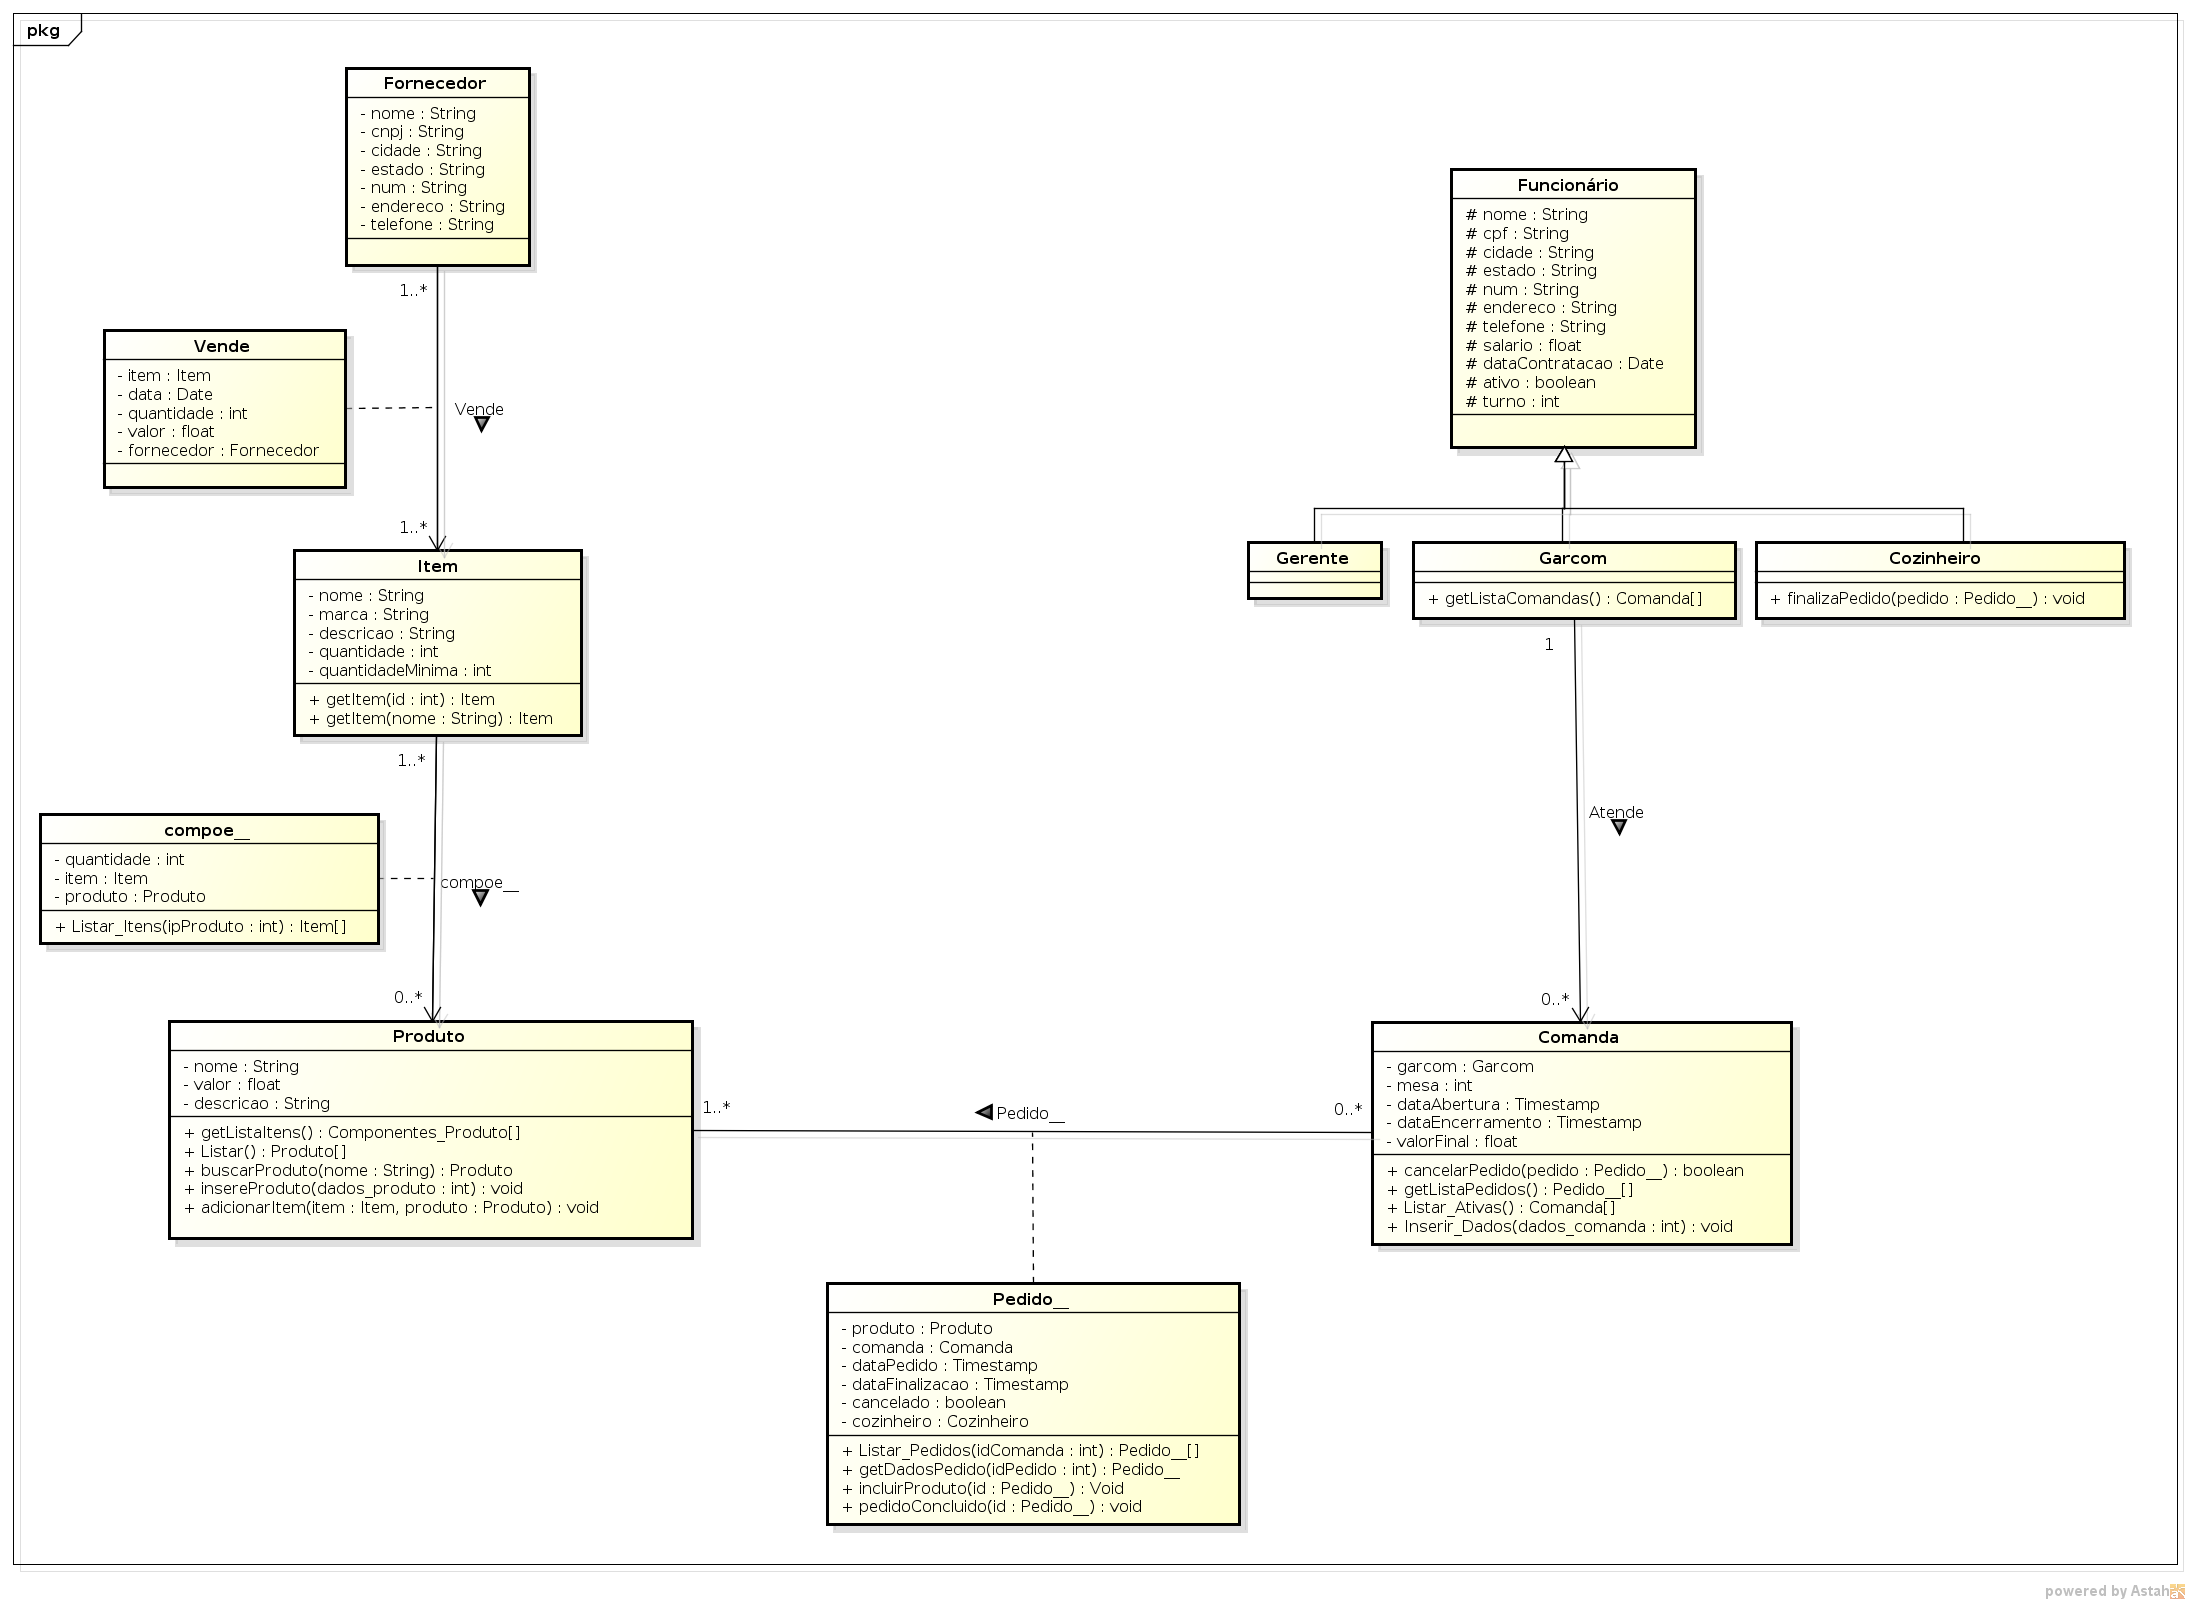
\includegraphics[scale=0.38,angle=90]{diagrama/Diagrama_de_Classe.png}
}
\let\cleardoublepage\clearpage
\newpage
\subsection{Diagrama de Classe de Projeto}
\centerline{
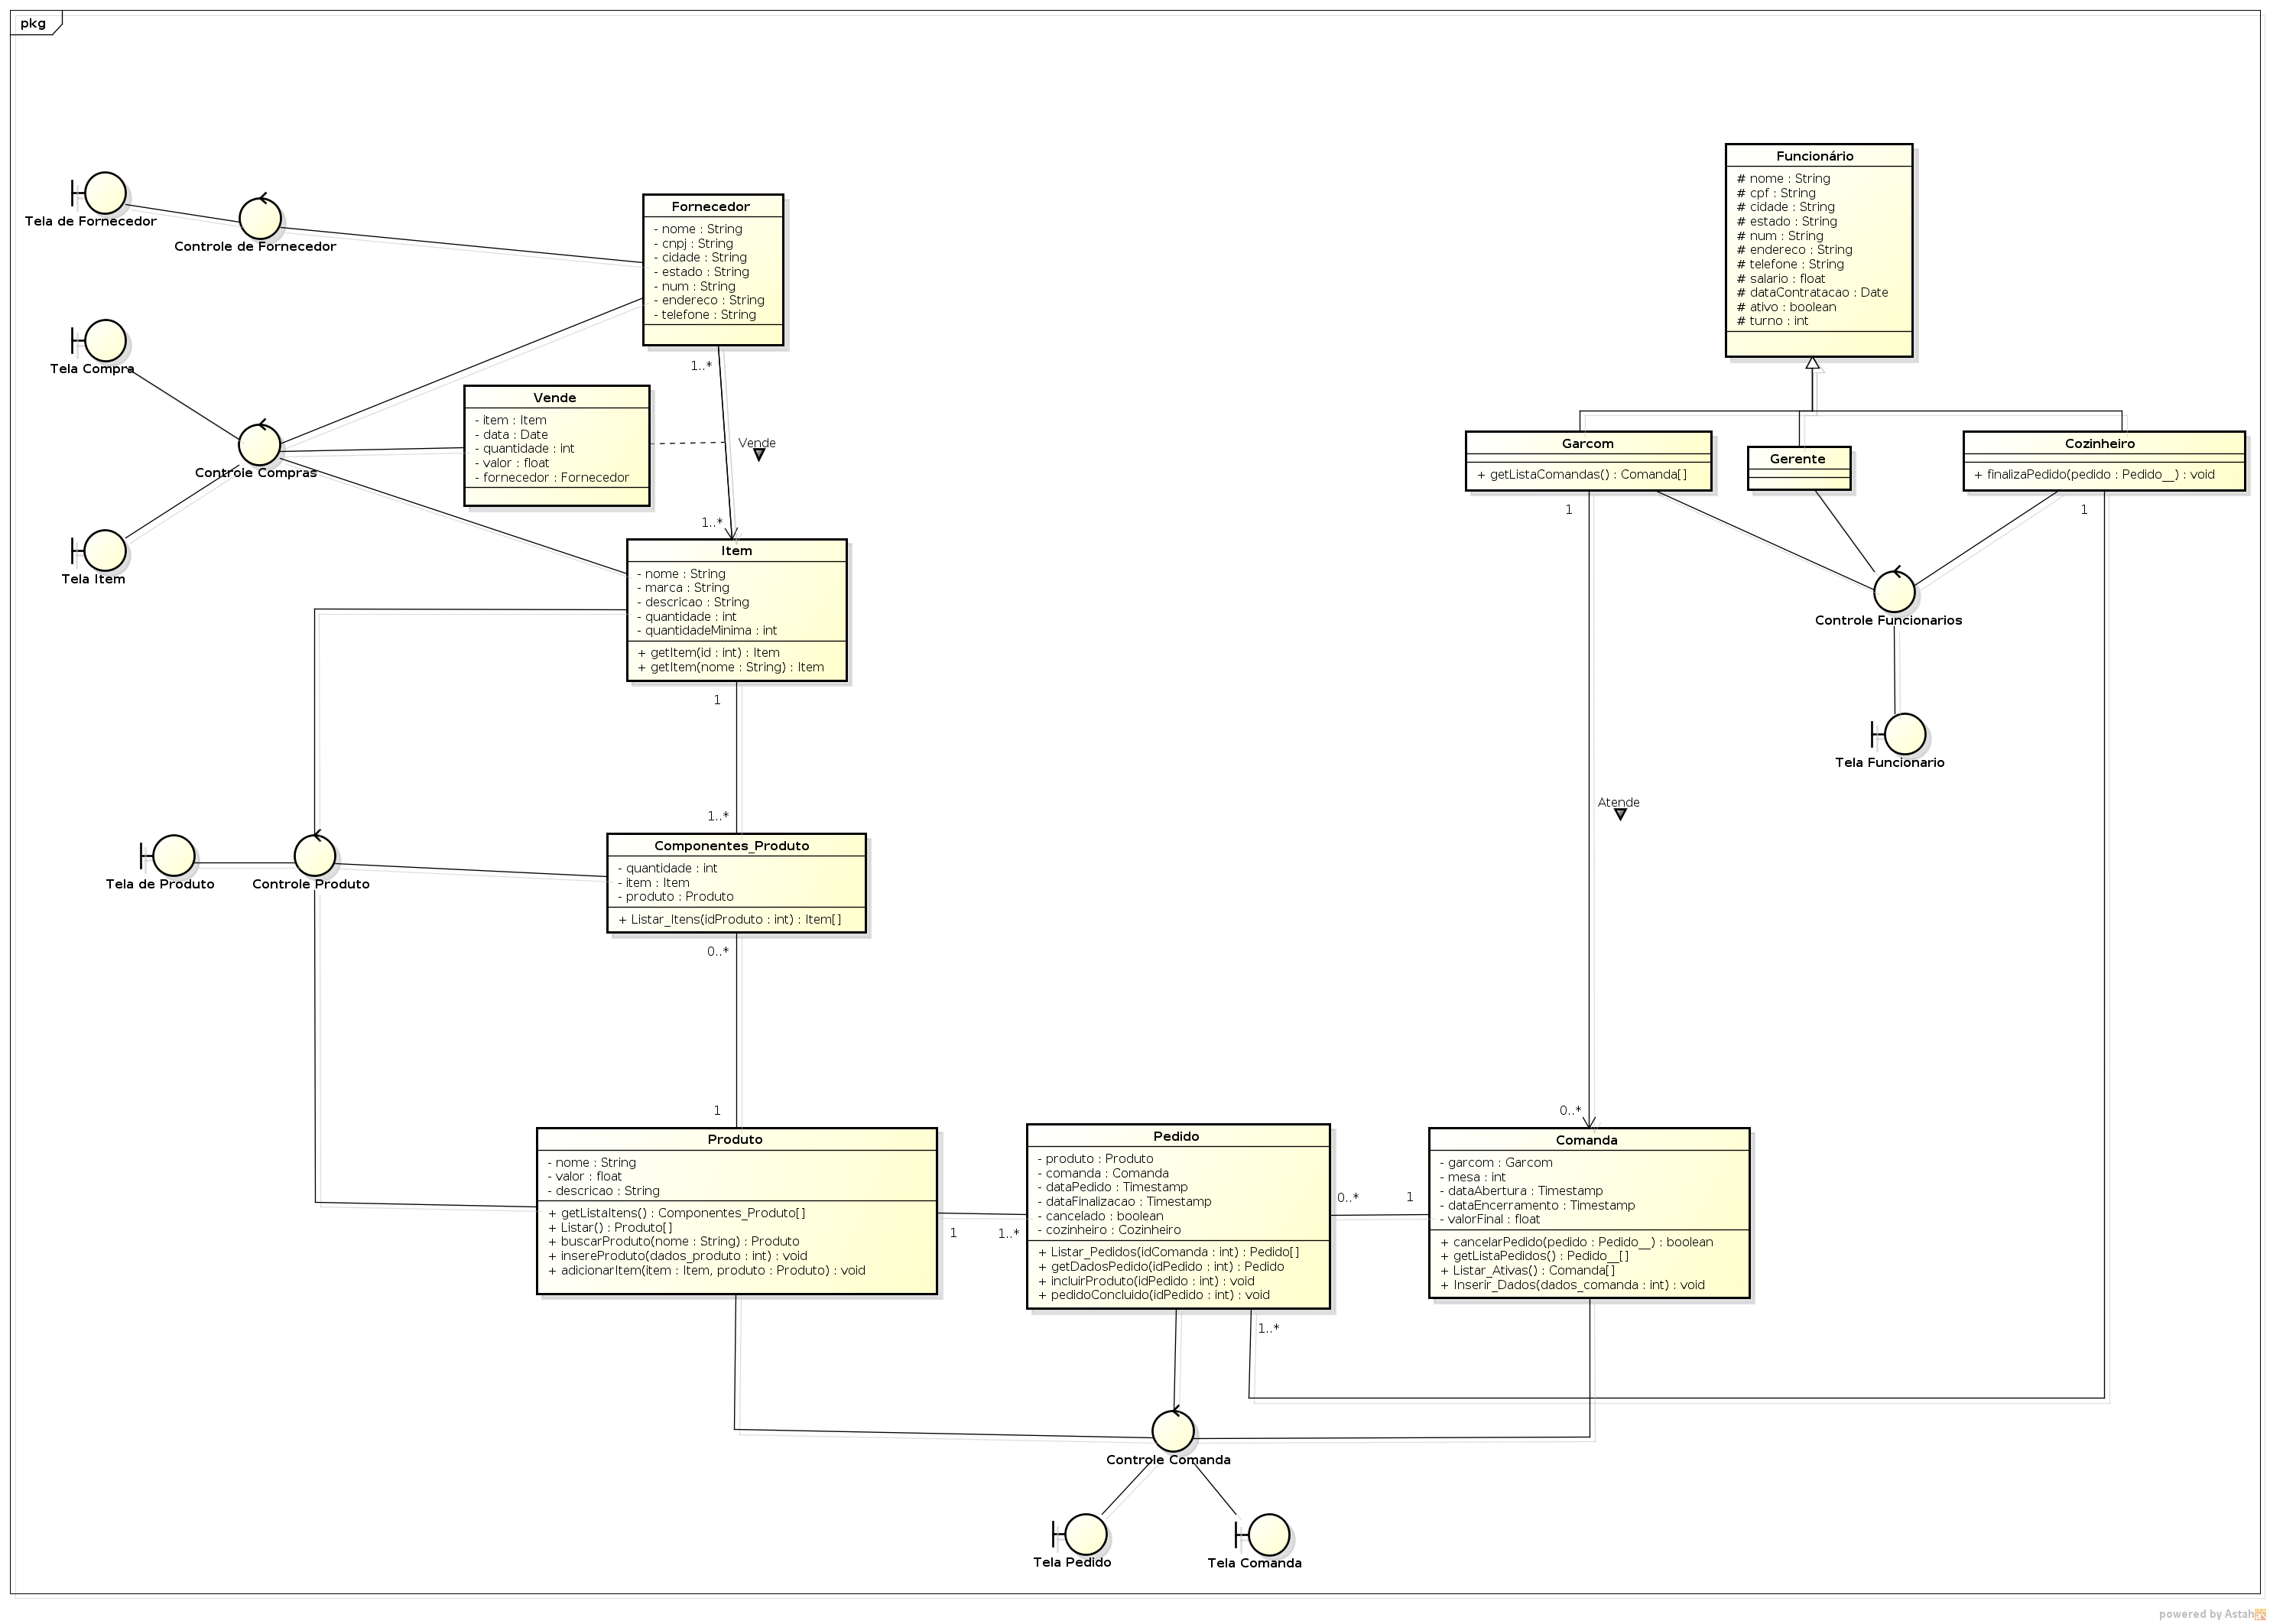
\includegraphics[scale=0.3,angle=90]{diagrama/Diagrama_de_Classe_Completo.png}
}

\newpage
\subsection{Diagrama de Atividade}

\subsubsection{Abertura e fechamento da comanda}
    \centerline{
      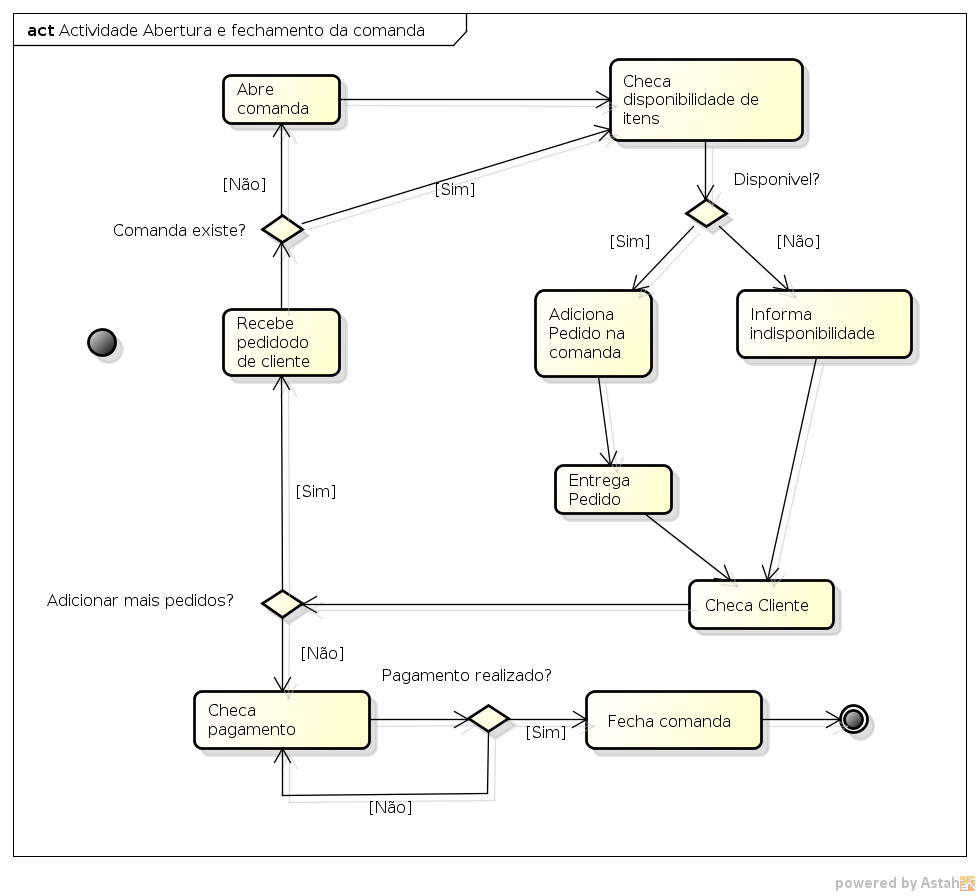
\includegraphics[scale=0.6]{diagrama/abertura_fechamento.png}
    }

\newpage
\subsubsection{Consultar informações de pedidos na comanda}
\centerline{
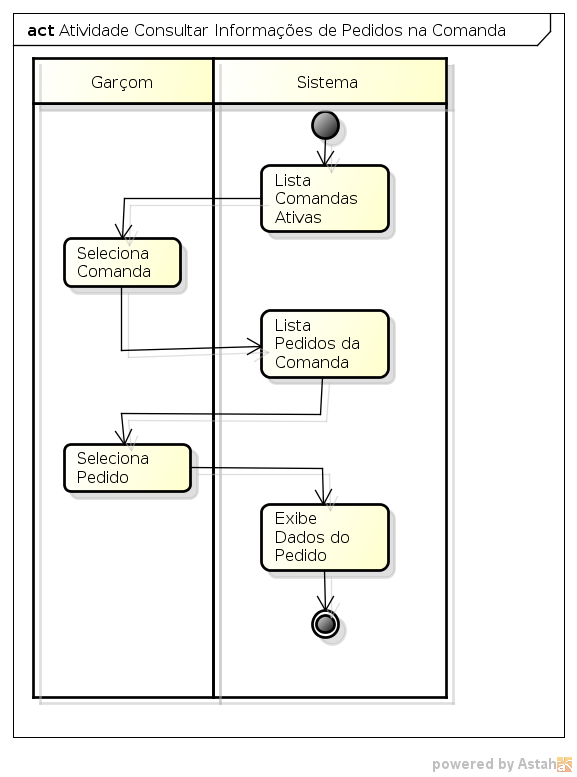
\includegraphics[scale=0.7]{diagrama/Atividade_Consultar_Informacoes_de_Pedidos_na_Comanda.png}
}

\newpage
\subsubsection{Inclusão de produto}
\centerline{
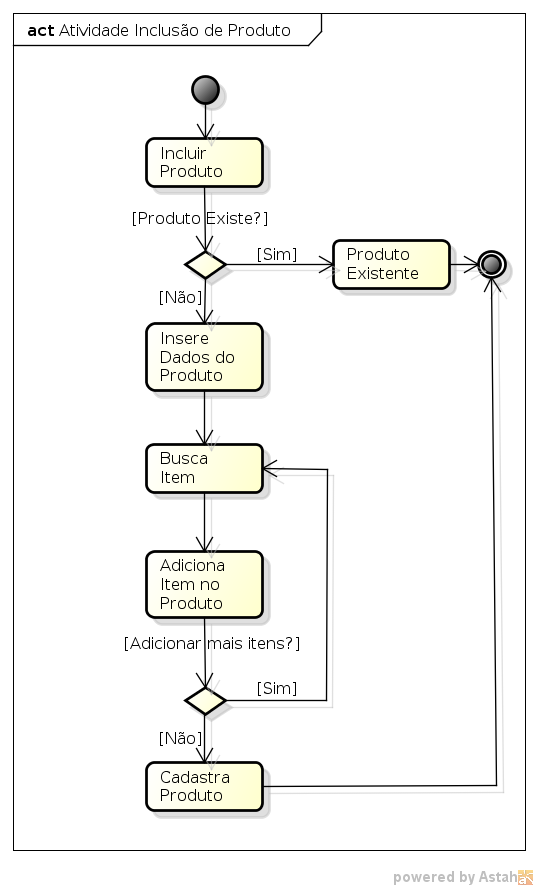
\includegraphics[scale=0.7]{diagrama/Atividade_Inclusao_de_Produto.png}
}
\let\cleardoublepage\clearpage
\newpage
\subsection{Diagrama de caso de uso}
\centerline{
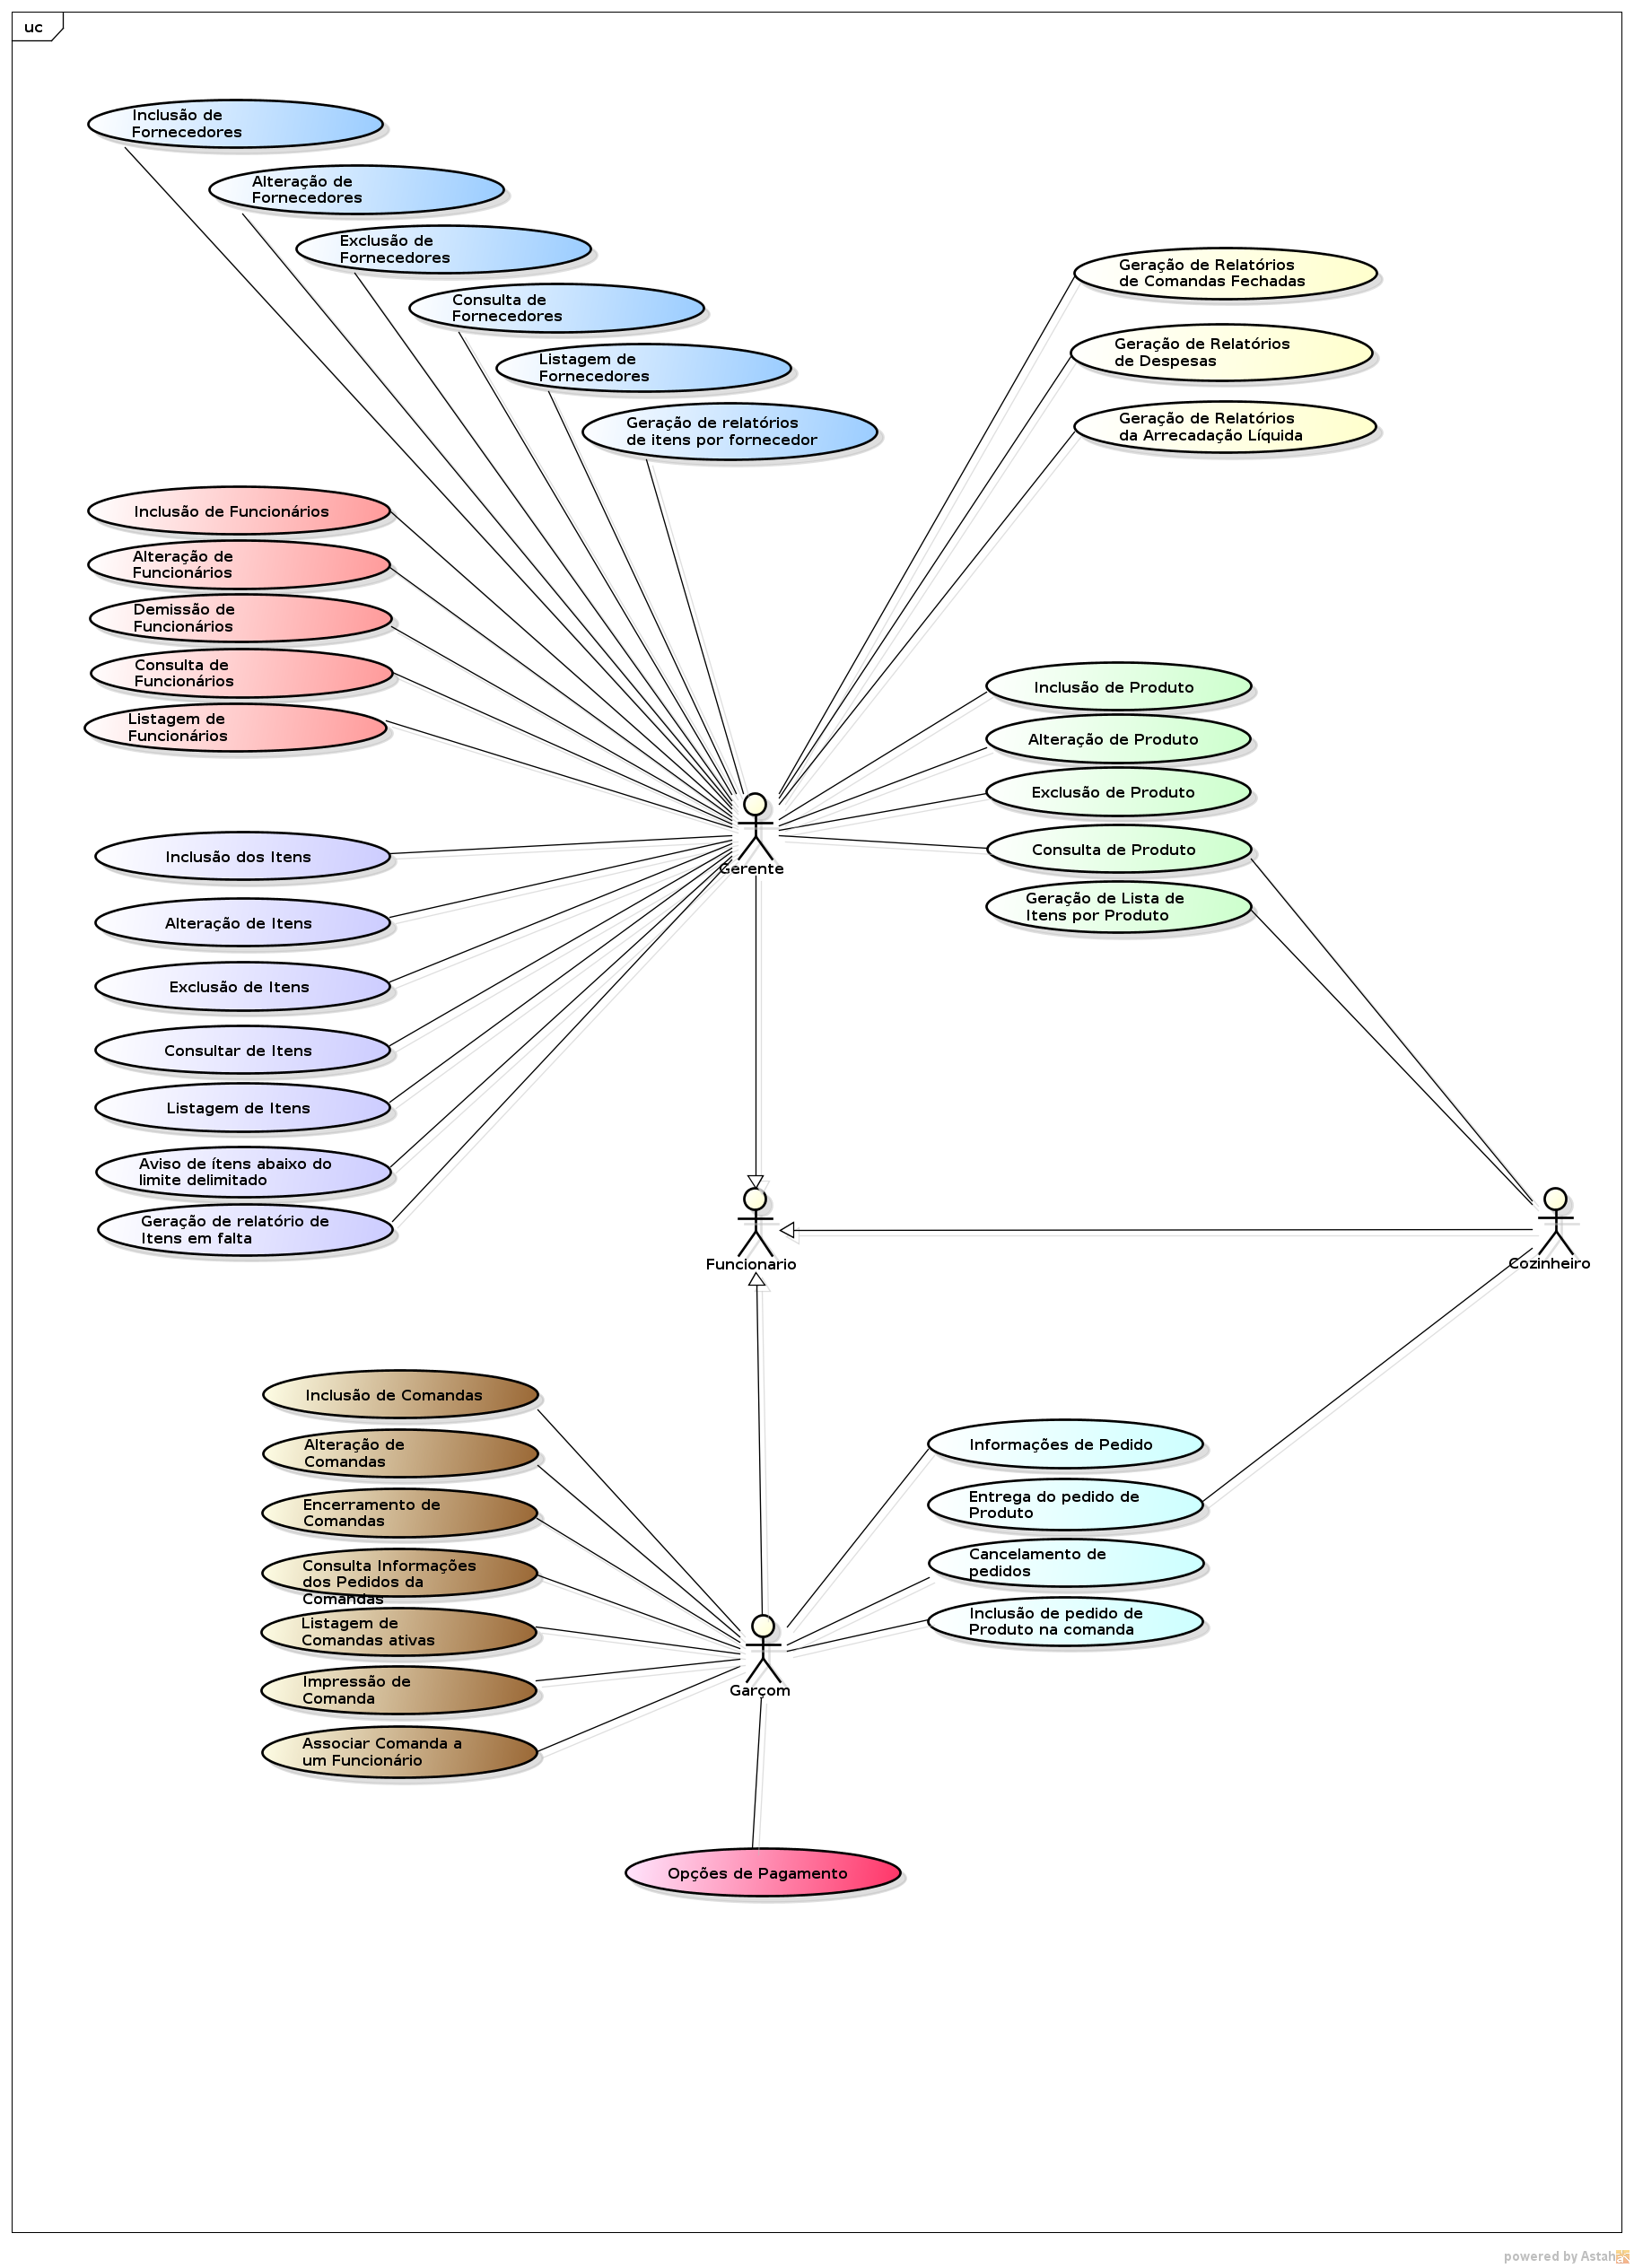
\includegraphics[scale=0.38]{diagrama/Diagrama_de_Caso_de_Uso.png}
}

\newpage
\subsection{Diagramas de Sequência}
\subsubsection{Consultar informações de pedidos na comanda}
\centerline{
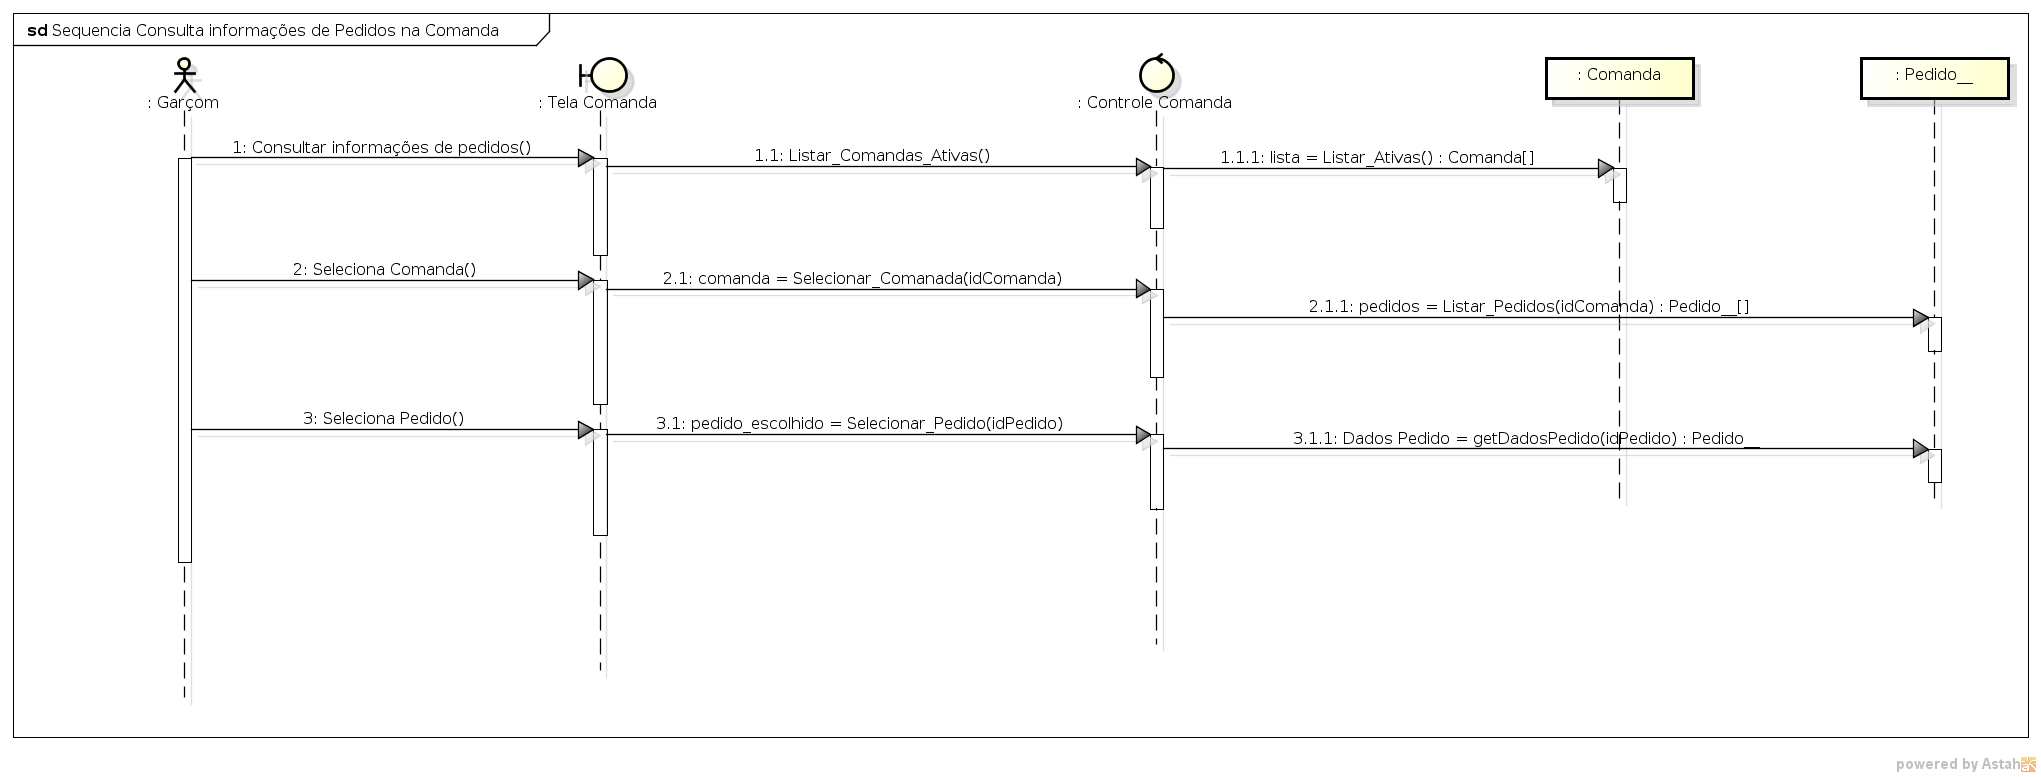
\includegraphics[scale=0.39,angle=90]{diagrama/sequencia_consulta_informacoes_de_pedidos_na_comanda.png}
}

\newpage
\subsubsection{Geração de Lista de itens por produto}
\centerline{
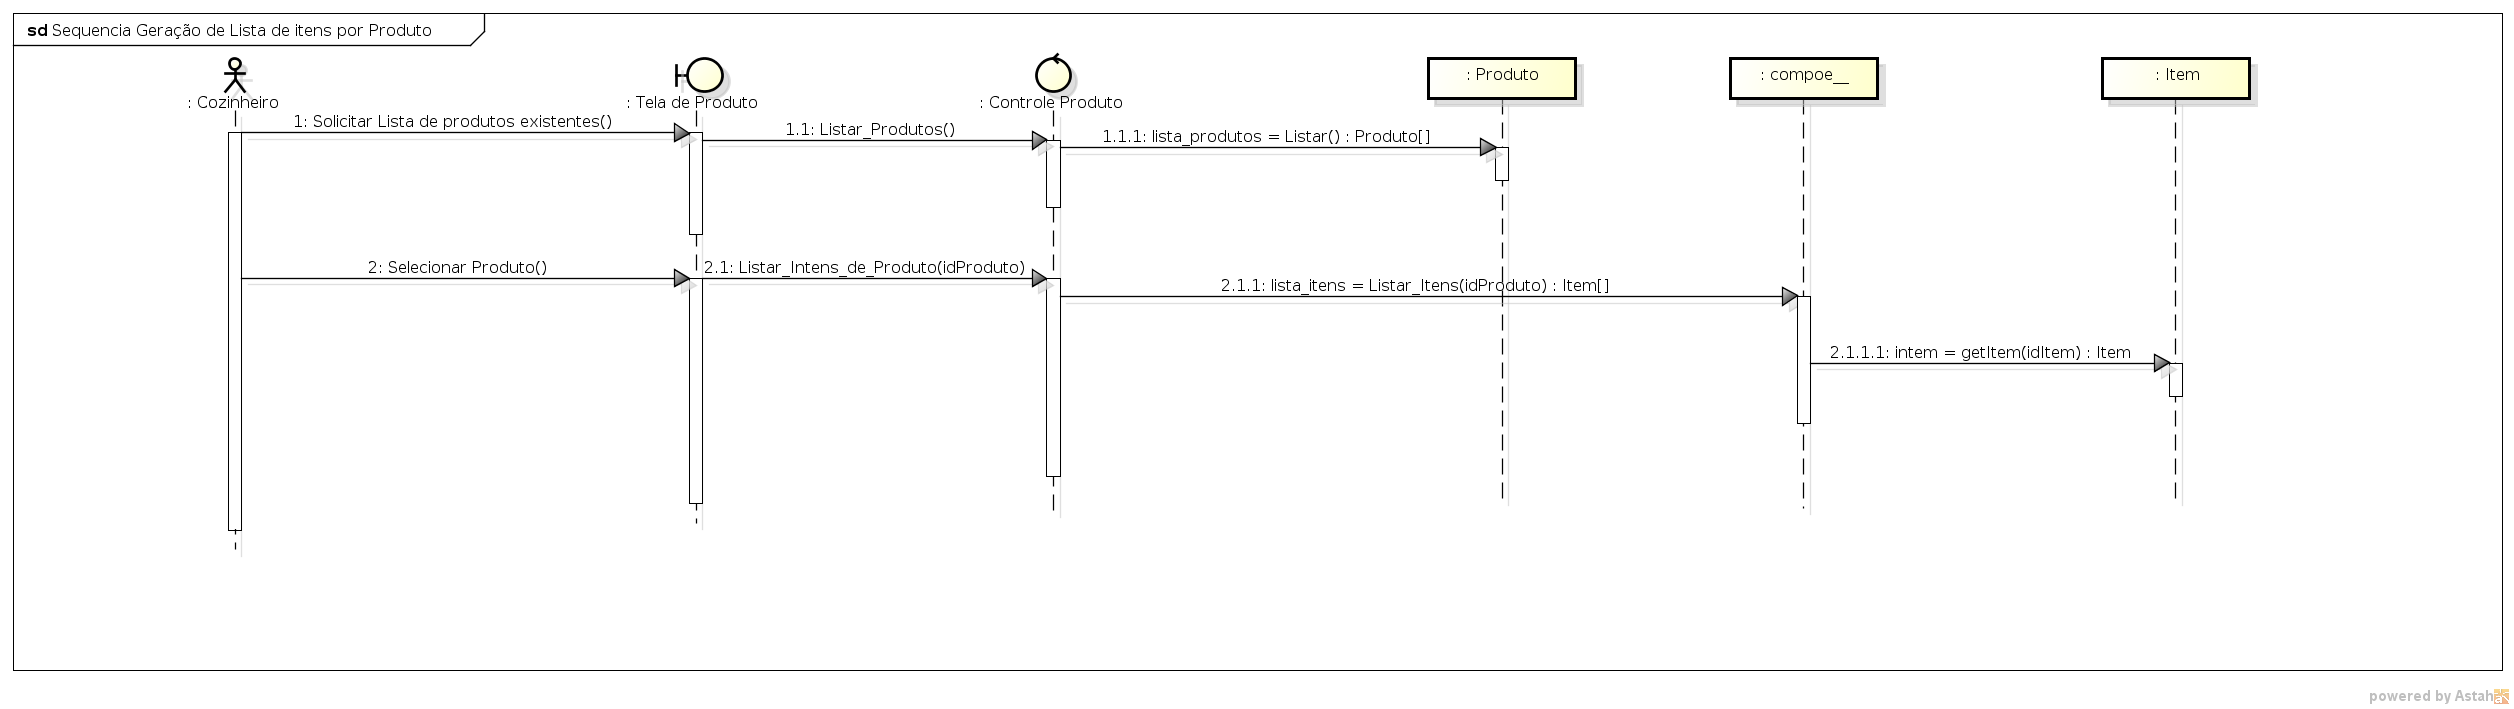
\includegraphics[scale=0.30,angle=90]{diagrama/sequencia_geracao_de_lista_de_itens_por_produto.png}
}

\newpage
\subsubsection{Inclusão de comanda}
\centerline{
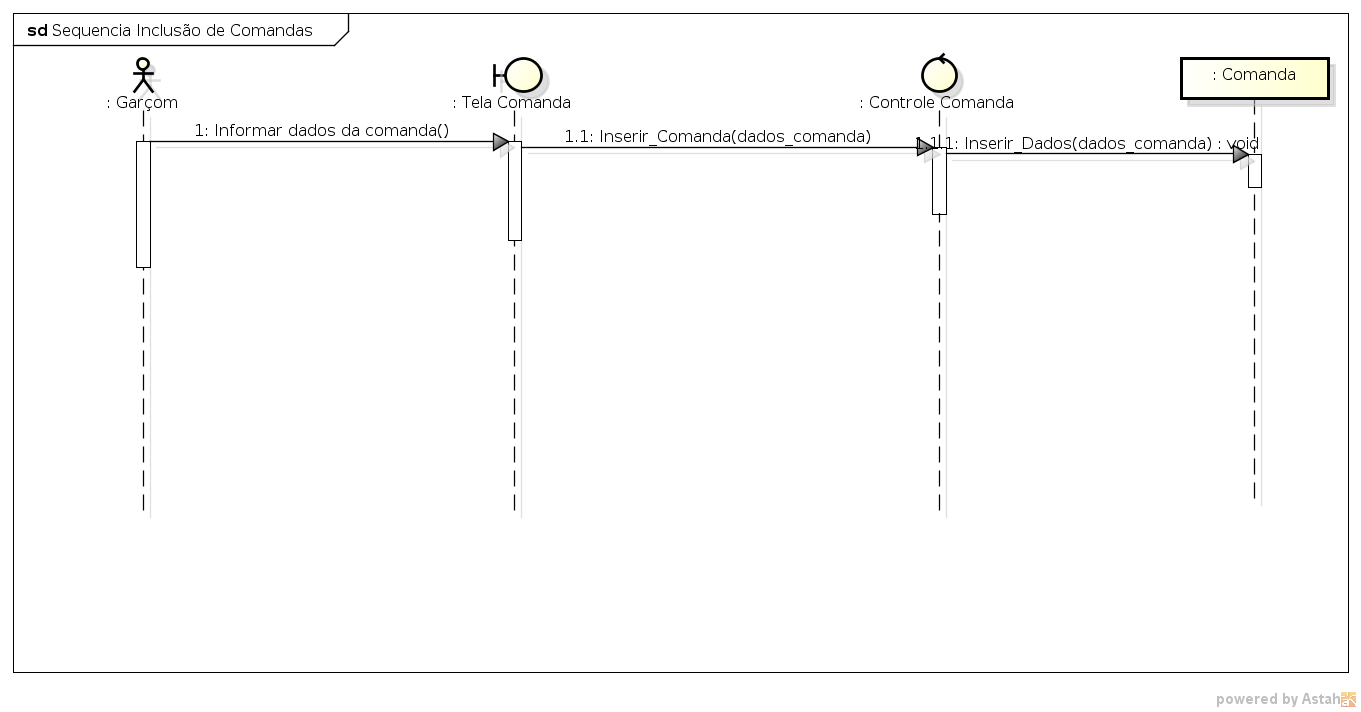
\includegraphics[scale=0.49,angle=90]{diagrama/sequencia_inclusao_de_comandas.png}
}


\newpage
\subsubsection{Inclusão de pedido na comanda}
\centerline{
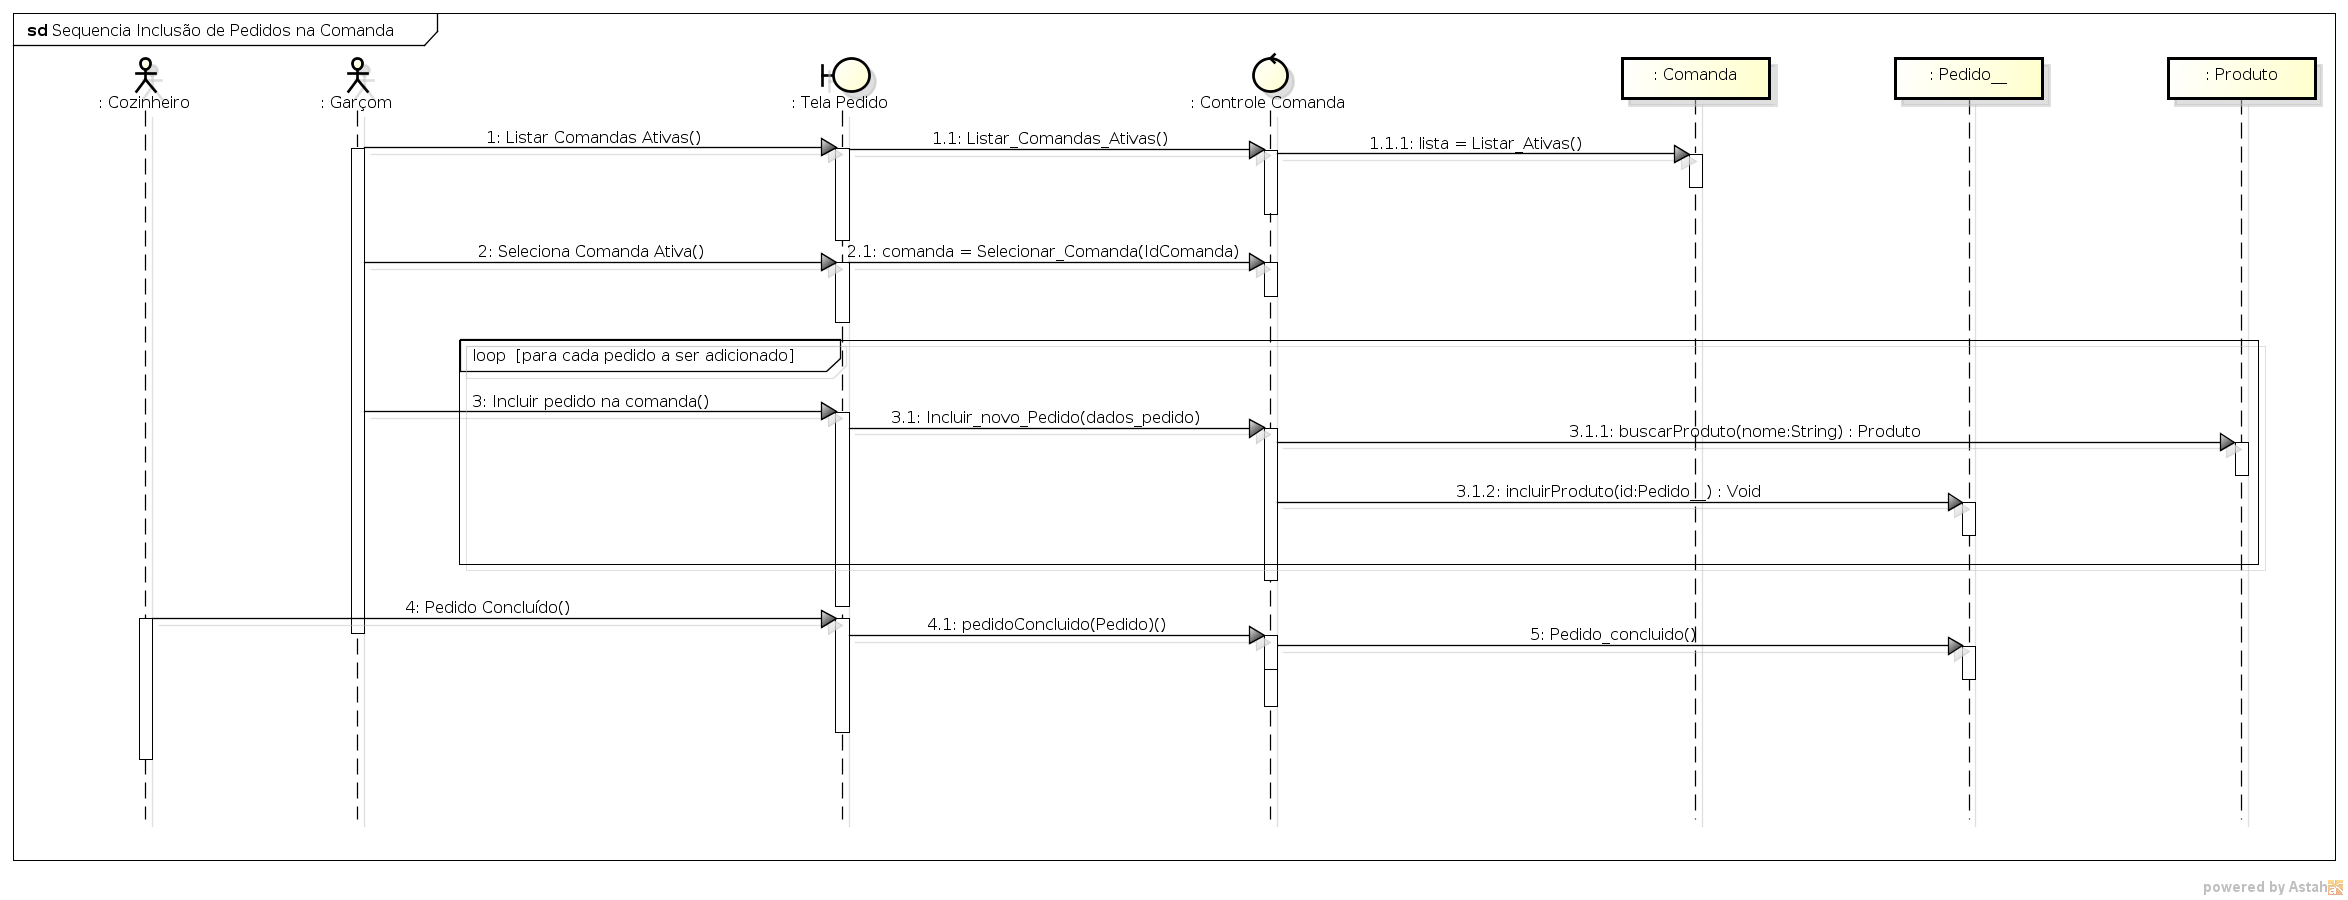
\includegraphics[scale=0.35,angle=90]{diagrama/Sequencia_Inclusao_de_Pedidos_na_Comanda.png}
}
\newpage
\subsubsection{Inclusão de produto}
\centerline{
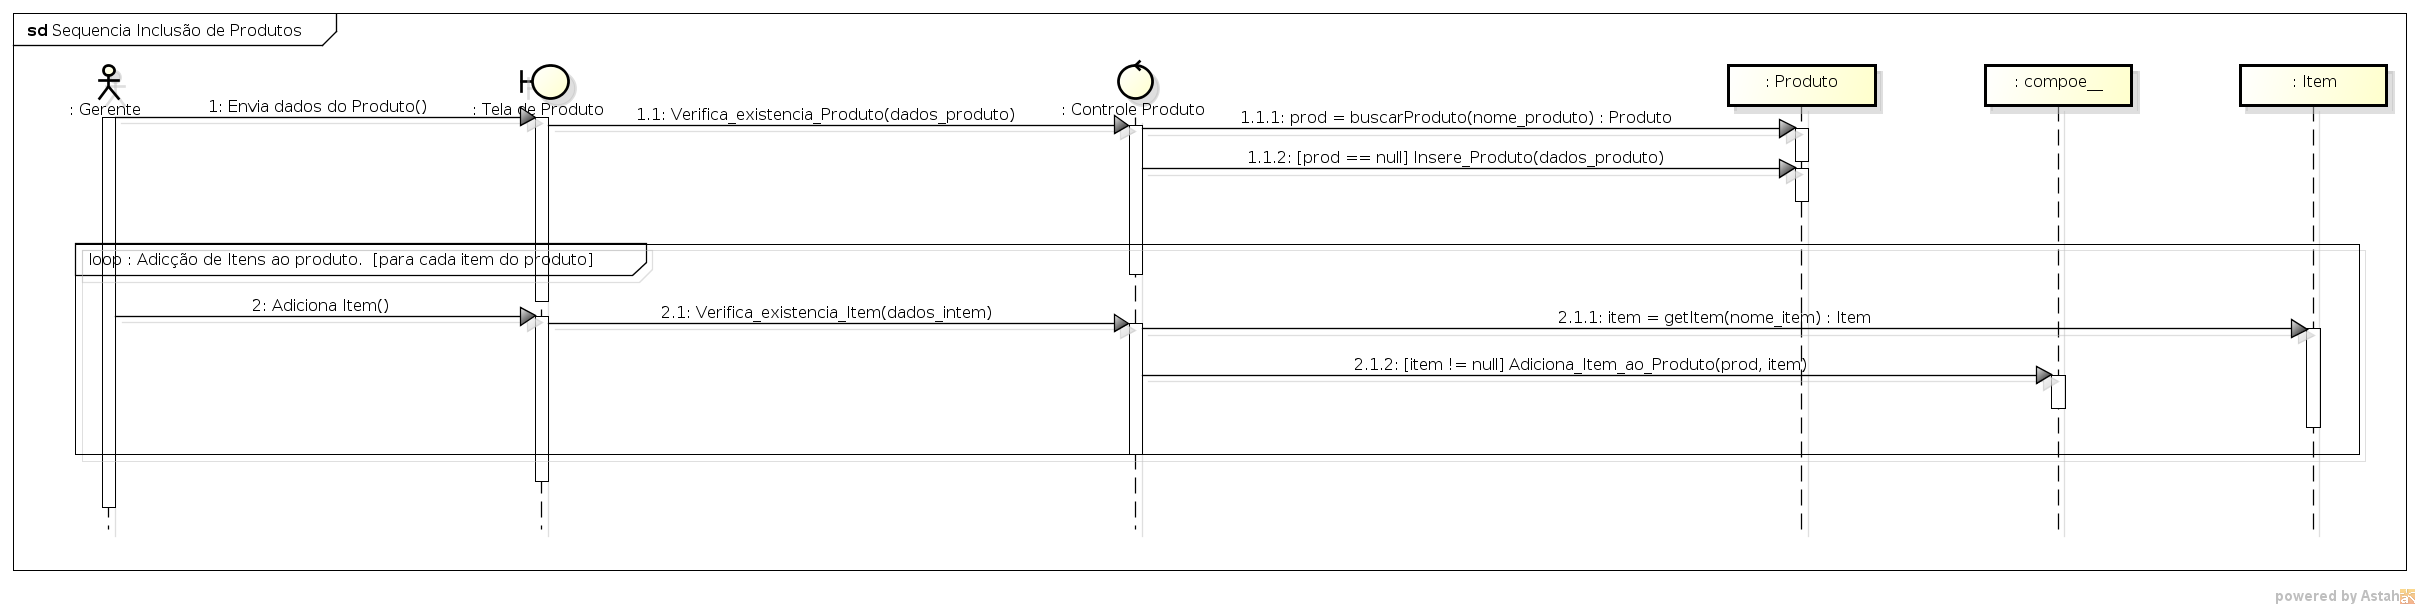
\includegraphics[scale=0.30,angle=90]{diagrama/Sequencia_Inclusao_de_Produtos.png}
}



\end{document}
